\chapter{Our representation for trips over urban streets}
	As explained in Section~\ref{sec:pd}, we have identified two contexts for public transportation systems according to their networks, which can be based on urban streets or public transportation. While the proposed structure in this chapter is capable of operating within both contexts, it will not take public transportation elements (routes and vehicles) into account and lead to a more redundant representation than the one later proposed in Chapter~\ref{sec:newctr}, that is more adequate for public transportation networks.
	
	The work in this chapter proposes a new structure named \gls{ctr} that answers  counting-based queries and uses compact self-indexed data structures to represent the large amount of trips in a compact space.
	\gls{ctr} combines two well-known data structures. The first one,
	initially designed for the representation of strings, is the
	\gls{csa}. The second
	one is the \gls{wt}. With these two structures, \gls{ctr} is able to efficiently resolve queries over trip patterns in any dimension (spatial, temporal or, combining both structures, spatio-temporal).

	We experimentally tested our proposal using two sets of %synthetic
	data representing trips over two different real public
	transportation systems. Our results are promising because the
	representation uses around  $50$\% of its original size and
	answers most of our spatial, temporal,  and spatio-temporal queries within $1\!-\!1000$ microseconds. 
	No experimental comparisons with classical spatial or spatio-temporal
	index structures were possible, because none of them were designed to
	answer the types of queries in this work. Our approach can  be
	considered as a proof of concept that opens new application
	domains for the use of well-known compact data structures such as the
	\gls{csa} and the \gls{wt}, creating a new strategy for
	exploiting trajectories represented in a self-indexed way.

\section{Description}
\label{sec:ctr_desc}
    Given a transportation network, whether it is based on urban strets or public transportation, we work with a representation of the network that is based on a directed graph. For an urban street network, a \textbf{node} represents a road segment delimited by intersections, where two nodes are connected by an edge if it is possible (i.e. legally allowed). This allows to accurately describe a trajectory by sequentially listing the road segments that were traversed, while minimizing the redundancy.

	In the other hand, for public transportation networks we define the nodes as stops or stations, making two of them connected if there exists a line or route that stops at each, consecutively. We can represent user trajectories following the same strategy as for urban street networks, although that will lead us to redundant representations in most cases. On subway and bus networks it is common to find stops that belong to only one route, and therefore must be either the end of a trajectory or be followed by the only possible next node. Furthermore, a more minimalist representation of a trajectory with the starting, ending and route switching nodes alone would be sufficient to reconstruct the original trajectory. Such representation will be contemplated later in Chapter~\ref{sec:newctr}, while on \gls{ctr} we maintain a common representation strategy for both kinds of networks. Because listing every node traversed introduces redundancy on public transportation networks, we state that \gls{ctr} is more adequate for urban street networks.
	
	\begin{figure}[ht]
		\begin{center}
			{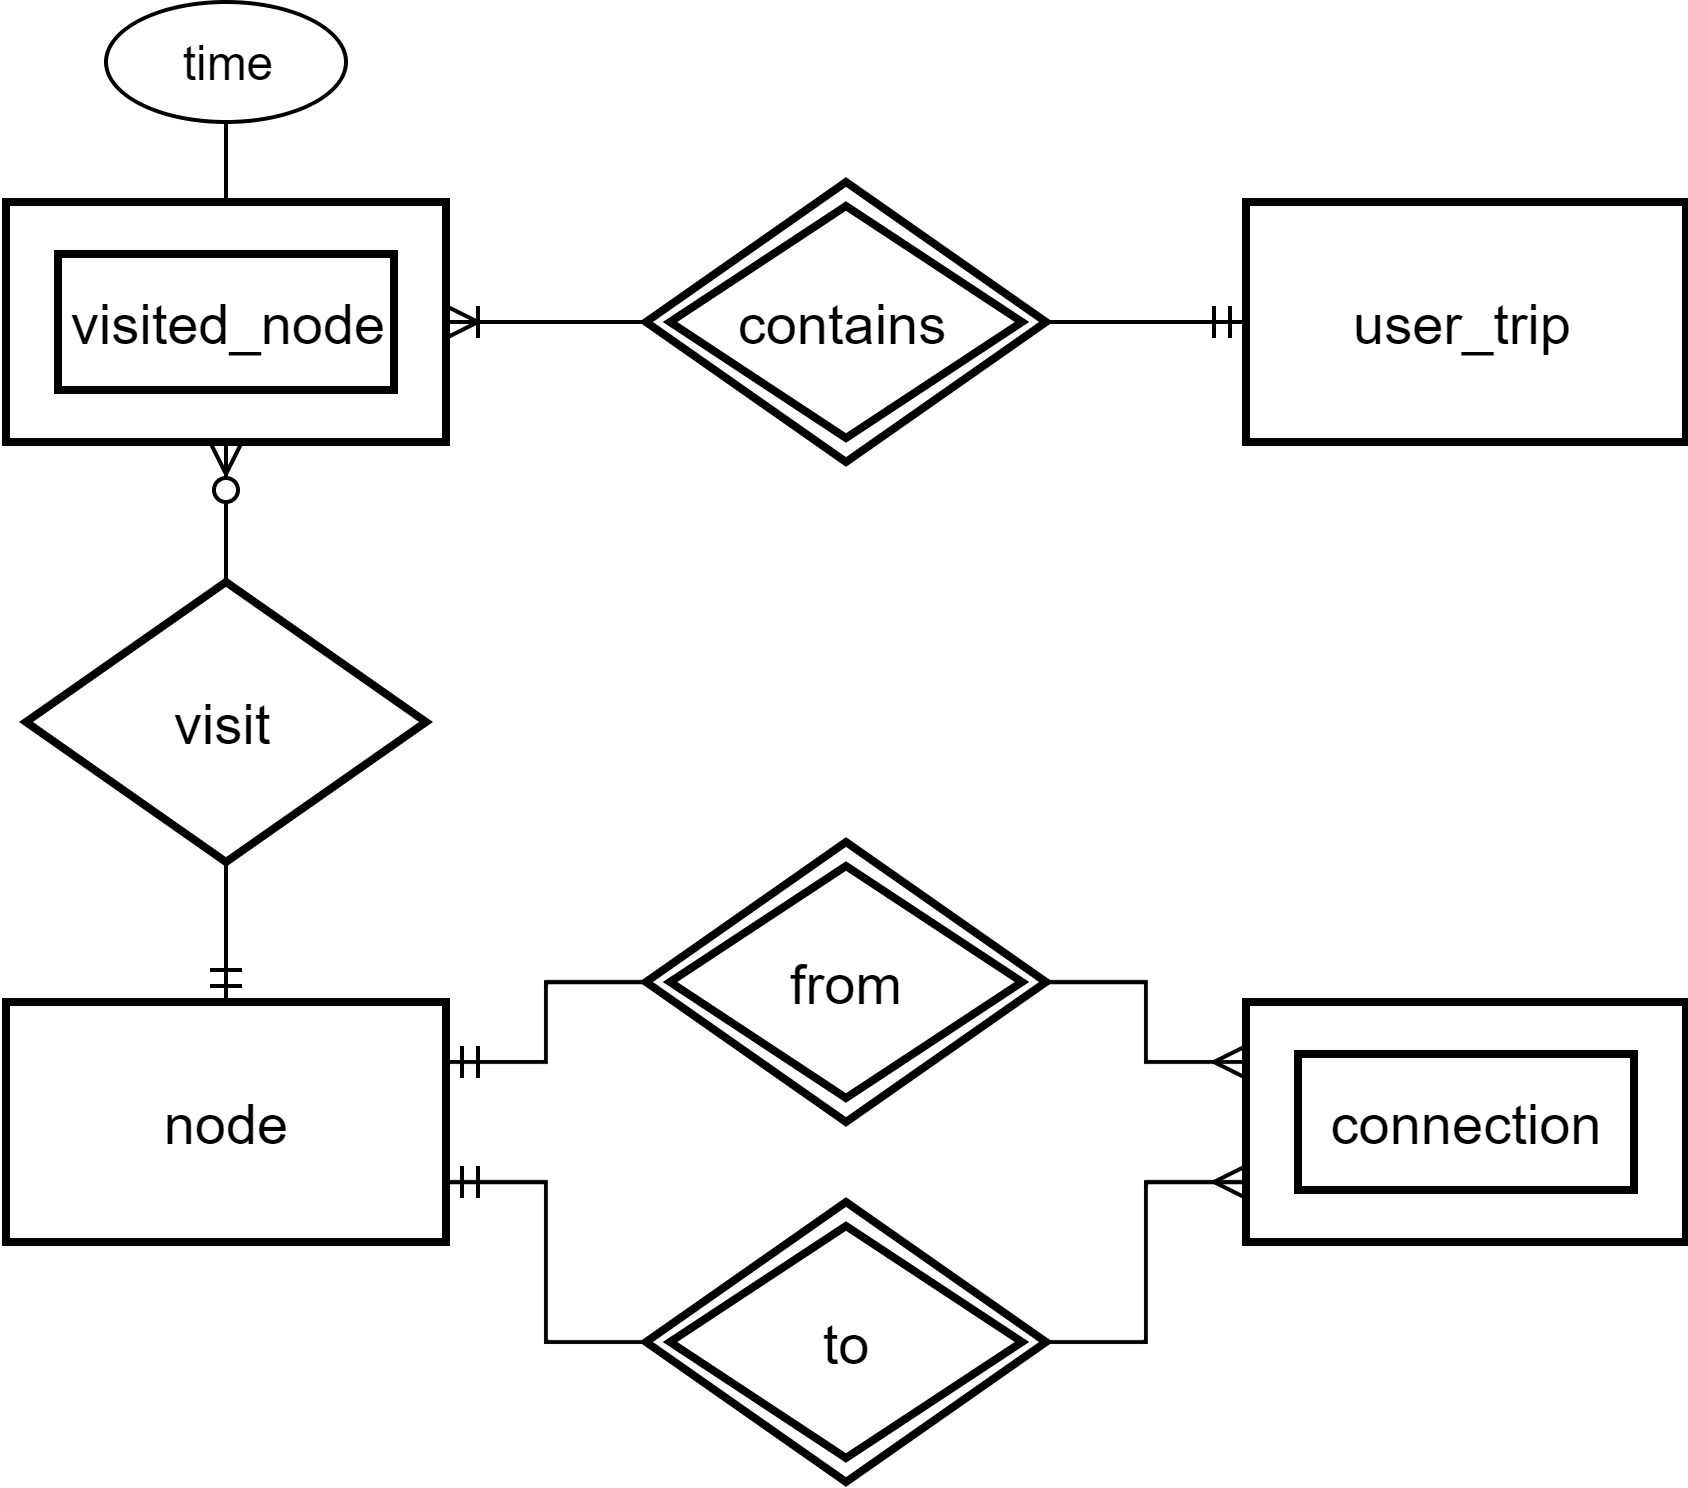
\includegraphics[width=0.6\textwidth]{figures/street_er.png}}
		\end{center}
		\caption{An ER diagram representing the model for user trips for \acrshort{ctr}}
		\label{fig:street_er}
	\end{figure}
    
    The Figure~\ref{fig:street_er} contains an entity-relationship diagram of our network model, where nodes and connections define a directed graph, over which user trips can be conformed by sequentially visiting the nodes. The order in which these nodes are visited is implicitly defined by the time, meaning that it is necessary to somehow represent that time for the visited nodes of each trip.
    It is easy to see how this model could introduce redundancy in the public transportation context, where several passengers may be sharing the same bus at the same time.
	
	To make the
	use of the \gls{csa} possible, we define a trip or trajectory of a moving object
	over a network as the temporally-ordered sequence of the nodes the trip
	traverses. An integer $s_i \in S$ is assigned to each node such that a trip is a sequence (string) of consecutively visited nodes by a single user. Note that this representation avoids the cost of storing coordinates to represent the location users pass through during a trip. It is just enough to identify the stops or nodes and when necessary to map these nodes to geographic locations. Moreover, when the underlying network is formed by street segments, we do not specify at which part of the segment did the trip start or finished: we consider such level of detail irrelevant for traffic analysis, as it can be effectively made on a street-segment level.
	
	We then build a \gls{csa}, over the concatenation of
	these strings (trips), with some adaptations for this
	specific application. In addition, we discretize the time in periods of fixed
	duration (i.e. timeline split into 5-minute intervals) and each time
	segment is identified by an integer $t_i \in I$. In this way, it is possible
	to store the times when trips reach each node by associating the
	corresponding $t_i$ with each node in each trip. The sequence of
	times for all the nodes within a trip is self-indexed with a \gls{wt}
	to efficiently answer temporal and spatio-temporal queries.

	Among other types of queries, in this work we focus on the following counting queries, which to the best of our knowledge have not been  addressed by previous proposals. In general terms, we define two general queries, number-of-trips queries and top-k queries, upon which we apply spatial, temporal or spatio-temporal constraint when useful.

	\begin{itemize}
		\item[(a)] {\em Number-of-trips queries.} This is a general type of queries that counts the number of distinct trips. When applying spatial, temporal or spatio-temporal constraints, it can specialized in the following queries:
		
		\begin{enumerate}
			\item Pure spatial queries:
			\begin{itemize}
				\item[-] {\em Number of trips starting at node $X$ (\startX).}
				\item[-] {\em Number of trips ending at node $X$ (\endX).} 
				\item[-] {\em Number of trips starting at $X$ and ending at $Y$ (\XtoY).}
				\item[-] {\em Number of trips using or passing through node $X$. Can also be seen as the average load of the node $X$. (\loadX)}
			\end{itemize}
			
			\item Spatio-temporal queries:
			\begin{itemize}
				\item[-] {\em Number of trips starting at node $X$ during time interval $[t_1,t_2]$ (\startX$_T$).}
				\item[-] {\em Number of trips ending at node $X$ during the time interval $[t_1,t_2]$ (\endX$_T$). }
				\item[-] {\em Number of trips starting at $X$ and ending at $Y$ occurring during  time interval $[t_1,t_2]$ (\XtoY$_T$).} This type of queries is further classified into: 
				\begin{itemize}
				    \item[(i)] \XtoY$_T$ with strong semantics (\XtoY$_{Ts}$), which considers trips that completely occur within interval $[t_1,t_2]$.
				    \item[(ii)] \XtoY$_T$ with weak semantics (\XtoY$_{Tw}$), which considers trips whose life time overlap $[t_1,t_2]$.
				\end{itemize}
				\item[-] {\em Number of trips using node $X$ during the time interval $[t_1,t_2]$. Can also be seen as the average load of the node $X$ within a given time interval. (\loadX$_T$).}
			\end{itemize}
			
			\item Pure temporal queries:
			\begin{itemize}
				\item[-] {\em Number of trips starting during the time interval $[t_1,t_2]$ (\startT). } 
				\item[-] {\em Total usage (load) of network stops during the time interval $[t_1,t_2]$ (\loadT).}
				\item[-] {\em Number of trips performed within the time interval $[t_1,t_2]$ (\tripT).} 
			\end{itemize}
		\end{enumerate}
		
		\item[(b)] {\em Top-k queries.} In this type of queries we want to retrieve the $k$ nodes with the highest number of trips. In this case, depending on having a temporal constraint or not we include the following queries:
		\begin{enumerate}
			\item Pure spatial {\em Top-k} queries:
			\begin{itemize}
				\item[-] {\em Top-k most used nodes (\topK)} that returns the nodes with the largest number of trips passing through.
				\item[-] {\em Top-k most used nodes to start a trip (\topK$_s$)} that returns the nodes with the largest number of trips that start at that node.
			\end{itemize}
			
			\item Spatio-temporal {\em Top-k}  queries:
			\begin{itemize}
				\item[-] {\em Top-k most used nodes during time interval $[t_1,t_2]$(\topK$_T$)} that returns the nodes with the largest number of trips passing through within time interval $[t_1,t_2]$. 
				\item[-] {\em Top-k most used nodes to start a trip during time interval $[t_1,t_2]$(\topK$_{Ts}$)} that returns the nodes with the largest number of trips starting there within time interval $[t_1,t_2]$ at that node.
			\end{itemize}
		\end{enumerate}
	\end{itemize}

\section{Structures}
\label{sec:ctr_str}
	To support the queries seen in Section~\ref{sec:ctr_desc}, we need to represent the spatial and temporal components of our collection of user trips that is coherent with the network model described. Therefore, we will proceed to detail how each trip is described, before we show how that description is implemented in our compact data structures.

	If we consider a network $\mathcal{N}$ with a set of nodes $S$, 
	we can see a dataset of trips $\mathcal{T}$ over $\mathcal{N}$ as 
	a set of trips, where for each trip $\mathcal{T}_i \in \mathcal{T}$, we represent a list with the 
	$n_i$
	temporary-ordered nodes it traverses and the corresponding timestamps: 
	$\mathcal{T}= \{ \langle (s^i_1, s^i_2, \dots,  s^i_{n_i}),(t^i_1, t^i_2, \dots,  t^i_{n_i}) \rangle\}$, $i\in[1,|\mathcal{T}|]$, 
	$s^i_j \in S$, and $t^i_{x} \leq t^i_y, \forall x < y$. 
	Note that every node in the network can be identified with an integer ID $S_i \in S$ and that, if we are interested in
	analyzing the usage patterns of the network, we will also be interested in discretizing time into 
	time intervals (i.e. 5-min, 30-min intervals). Therefore,
	we will have $|I|$ different time intervals that can also be identified with an
	integer ID ($t^i_j \in I$).

	The size of the time interval is a parameter for the time-discretizing process
	that can be adjusted to fit the required precision in each domain.
	For example, in a public
	transportation network where we could have data including five years of trips, one
	possibility would be to divide that five-years period into
	10-minute intervals hence obtaining a
	vocabulary of $|I|=5\times 365 \times 24 \times 60/10 = 262,800$ different intervals. 
	Other possibility would
	be to use cyclically annual 10-minute periods resulting in $|I|=262,800 / 5 = 52,560$. 
	However,  in public transportation networks, queries such
	as \textit{``Number of trips using the stop X on May 10 between 9:15 and 10:00''} may be not 
	as useful as queries such as \textit{``Number of trips using stop X on Sundays between 9:15 and
		10:00''}.
	% Therefore, it is more useful
	%to encode with the same codes the hours in working days on one hand and
	%hours in weekend in the other.
	For this reason, \gls{ctr} can adapt how the
	time component is encoded depending on the queries that the system must answer.

	\begin{figure}[ht]
		\begin{center}
			{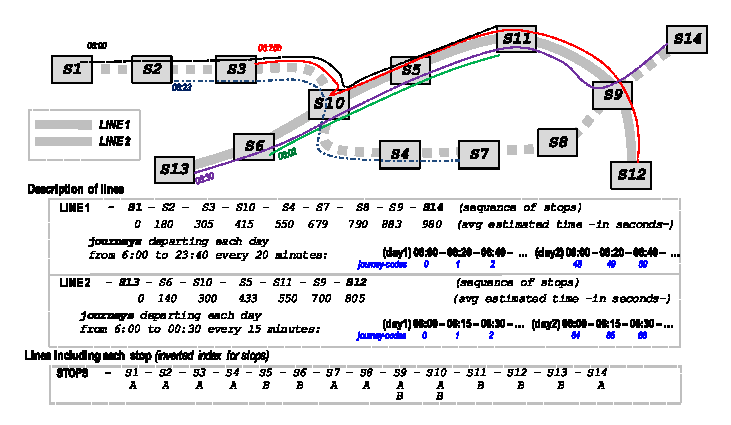
\includegraphics[width=1\textwidth]{figures/network.eps}}
		\end{center}
		\caption{A set of trips over a network with 10 nodes.}
		\label{fig:network}
	\end{figure}

	\begin{example} \label{exp:ctr}
	Figure~\ref{fig:network} shows a network that contains $|S|=10$ nodes 
	numbered from $1$ to $10$. Over that network we have six trips ($|\mathcal{T}|=6$),
	and, for each of them, we indicate the sequence of nodes it traverses
	and the time when the trip goes through those nodes. If we discretize time into
	5-minute intervals, starting at 08:00h, and ending at 9:20h, we will have
	have $|I|=16$ different time intervals. Any timestamp within
	interval $\mathit{[08\!:\!00,08\!:\!05)}$ will
	be assigned time-code $0$, those within $\mathit{[08\!:\!05,08\!:\!10)}$ code $1$, and so on until
	times within $\mathit{[09\!:\!15,09\!:\!20)}$ that are given time-code $15$.  
	Therefore, our dataset of trips will be: 
	$\mathcal{T}$: $\{$%
	$\langle (\mathbf{1,2,3     })$, $(\mathit{5,7,8})                     \rangle$, 
	$\langle (\mathbf{2,3,10,6  })$, $(\mathit{10,13,14,15})           \rangle$, 
	$\langle (\mathbf{1,2,3     })$, $(\mathit{0,3,5})                     \rangle$, 
	$\langle (\mathbf{2,3,10,4,7})$, $(\mathit{2,4,6,8,10}) \rangle$, 
	$\langle (\mathbf{3,10,5    })$, $(\mathit{9,11,12})                     \rangle$, 
	$\langle (\mathbf{9,8,7     })$, $(\mathit{12,14,15})                    \rangle$$\}$, 
	where bold numbers indicate node IDs and slanted ones indicate times. \qed
	\end{example}

	In \gls{ctr} we represent both the spatial and the temporal component of the trips using well-known
	self-indexing structures in order to provide both a compact representation and the ability to 
	perform fast indexed searches at query time. In Section~\ref{sec:transnet_repr} we focus on the
	spatial component and discuss how we adapted  \gls{csa} to deal with trips. We also
	show how we support spatial queries. Then, in Section~\ref{sec:time_repr} we show that the times,
	which are kept aligned with the spatial component of the trips, can be handled with   
	a \gls{wt}-based representation. Actually we study two alternatives (a \gls{htwt} and a \gls{wm}) 
	and show how temporal and spatio-temporal (Section~\ref{sec:stq}) queries are supported by \gls{ctr}.

	\subsection{Spatial component using a CSA}
	\label{sec:transnet_repr}
	We use a slightly adapted \gls{csa} to represent the spatial component of our dataset of trips within \gls{ctr}. 
	However, we must perform some preprocessing on each trip  $\mathcal{T}_i \in \mathcal{T}$ before building a \gls{csa} on it. Initially, we sort the trips by their first node ($s^i_1$), then by the last node ($s^i_n$), then by the starting time ($t^i_1$), and finally, by its second node ($s^i_2$), third node ($s^i_3$), and successive nodes (i.e. the trips are sorted by the key $s_1,s_n,t_1,s_{2..n-1}$.  Note that the start time ($t^i_1$) of the trip does not belong to the spatial component, but it is nevertheless used for the sorting\footnote{This initial sorting of the trips will allow us to answer some useful queries very efficiently  (i.e., count trips starting at node $X$ and ending at node $Y$).}.

	Following with Example~\ref{exp:ctr}, after sorting the trips in $\mathcal{T}$ with the criteria above, 
	our sorted dataset $\mathcal{T}^s$ would look like: 
	$\mathcal{T}^s$: $\{$%
	$\langle (\mathbf{1,2,3     })$, $(\mathit{0,3,5})                     \rangle$, 
	$\langle (\mathbf{1,2,3     })$, $(\mathit{5,7,8})                     \rangle$, 
	$\langle (\mathbf{2,3,10,6  })$, $(\mathit{10,13,14,15})           \rangle$, 
	$\langle (\mathbf{2,3,10,4,7})$, $(\mathit{2,4,6,8,10}) \rangle$, 
	$\langle (\mathbf{3,10,5    })$, $(\mathit{9,11,12})                     \rangle$, 
	$\langle (\mathbf{9,8,7     })$, $(\mathit{12,14,15})                    \rangle$$\}$. 
	Note that  $ (\mathbf{2,3,10,6  })$ appears before $(\mathbf{2,3,10,4,7})$ because
	during the sorting process we compare $ (\mathbf{2,6,\mathit{2},3, 10,6  })$ with $ (\mathbf{2,7,\mathit{10},3, 10,4,7})$;
	that is, we compare the starting nodes ($\mathbf{2}$ and $\mathbf{2}$) and then the ending nodes ($\mathbf{6}$ and $\mathbf{7}$).
	If needed  (not in this example) we would have also compared the slanted values ($\mathit{2}$ and $\mathit{10}$) 
	that are the starting times of the trips, and finally the rest of nodes  ($ \mathbf{3, 10,6  }$ and $ \mathbf{3, 10,4,7}$).
	Similarly, the two trips containing nodes $ (\mathbf{1,2,3})$ are sorted by the starting times ($\mathit{0}$ and $\mathit{5}$).


	In a second step, we enlarge all the trips $\mathcal{T}^s_i \in \mathcal{T}^2$ with a fictitious terminator-node $\$_i$ whose
	timestamp is set to that of the initial node of the trip. We choose terminators such that $\$_i \prec \$_j, \forall i<j$; 
	that is the lexicographic value of $\$_i$ is smaller for smaller $i$ values. In addition, the lexicographic value
	of any terminator must be lower than the ID of any node in a trip. Therefore, an enlarged trip $\mathcal{T}^s_i$
	would become $\mathcal{T}'_i =  \langle (s^i_1, s^i_2, \dots,  s^i_{n_i}, 
	\mathbf{\$_i}),(t^i_1, t^i_2, \dots,  t^i_{n_i}, \mathbf{t^i_1}) \rangle$. 

	The next step involves concatenating the codes $s^i_j$ and $\$_i$ of the spatial components of our trips and to add an 
	extra trailing terminator $\$_0$ to create a sequence $Text[1,n]$\footnote{By definition, it must hold that $n = |\mathcal{T}| + 1 + \displaystyle\sum^{|\mathcal{T}|}_{i=1} n_i$.}. $\$_0$ must be  lexicographically 
	smaller than any other entry in $S$ (then it also holds $\$_0 \prec \$_i$ $\forall i \in [1,|\mathcal{T}|]$). In the top part of
	Figure~\ref{fig:tcsa}, we can see array $Text$ for the running example, as well as the corresponding time-IDs that
	are regarded in sequence $Icode$  ($Time$ shows the original times).
	
	\begin{figure}[ht]
	  \begin{center}
	  {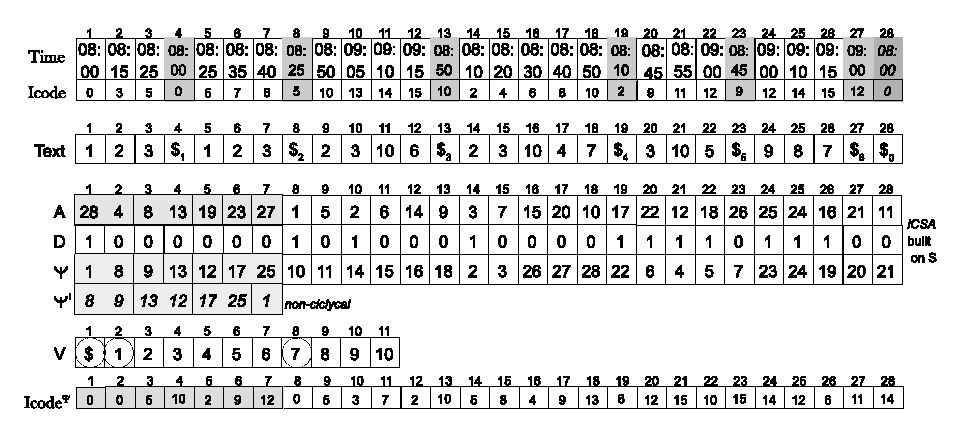
\includegraphics[width=1.00\textwidth]{figures/csttr.eps}}
	  \end{center}
	  \caption{Structures involved in the creation of a \acrshort{ctr}}
	  \label{fig:tcsa}
	\end{figure}

	Finally, we build a \gls{csa} on top of $Text$ to obtain a self-indexed representation of the spatial component in \gls{ctr}.
	Figure~\ref{fig:tcsa} depicts the structures $\Psi$ and $D$ used by the \gls{csa} built over $Text$. There is also a vocabulary
	$V$ containing a $\$$ symbol and the different node IDs in lexicographic order.

	Note that the use of different values $\$_i$ as terminators ensures that our sorting criteria are kept even if we follow the
	standard suffix-sort procedure\footnote{Suffix $Text[i..n]$ is compared with suffix $Text[j..n]$.} 
	required to build suffix array $A$ during the creation of \gls{csa}. Yet, when we finish that
	process, we can replace all those $\$_i$ terminators by a unique $\$$. This is the reason why there is only one $\$$ symbol in $V$. 
	 
	%while in $V$ there is only one single entry for all the $\$$. 
	%The use of different values for $\$_i$ during the sorting explains why $A[22] = 18$ is placed before $A[23]= 26$. Note that
	%the suffix starting at $S[18]$ is ``$7 \cdot \$_4 \cdot 2 \cdot 3 \dots$'' and that suffix at
	%$S[26]$ is ``$7 \cdot \$_6 \cdot 9 \cdot \dots$''. Therefore, it holds that $A[22] \prec A[23]$. However, considering
	%the traditional definition of a {\em suffix}, these suffixes would be ``$7 \cdot \$_4 \cdot 3 \cdots $''
	%and ``$7 \cdot \$_6 \cdot \$_0 \cdots $'' respectively,  and  $A[22] \prec A[23]$ would not hold.

	Although they are not needed in \gls{ctr}, we show also suffix array $A$ and $\Psi$' for clarity reasons in Figure~\ref{fig:tcsa}. 
	$\Psi'$  contains the first entries of $\Psi$ from a regular \gls{csa}, whereas we introduced a small variation
	in \gls{ctr} for entries $\Psi[1..|\mathcal{T}|+1]$. Displaying both $\Psi$ and $\Psi'$ helps us to better illustrate our process to build $\Psi$. 
	For example, $A[8]=1$ points to the first node of the first trip $S[1]$.
	$\Psi[8]=10$ and $A[10]=2$ point to the second node.  $\Psi[10]=14$ and $A[14]=3$ point to the third node.
	$\Psi[14]=2$ and $A[2]=4$ point to the ending $\$_1$ of the first trip. Therefore, in the standard 
	\gls{csa}, $\Psi'[2]=9$ and $A[9]=5$  point to the first node of the second trip. 
	However, in  \gls{ctr}, $\Psi[2]=8$ and $A[8]=1$ point
	to the first node of the first trip. With this small change, subsequent applications of $\Psi$ will allow 
	us to cyclically traverse the nodes of the trip instead of accessing the following entries of $Text$.

	Another interesting property arises from the use of a cyclical $\Psi$ on trips, and from using trip terminators.
	Since the first entries in $\Psi[2,|\mathcal{T}|+1]$ correspond the $\$$ symbols that 
	mark the end of each trip in $Text$ (remember that $\Psi[1]$ corresponds the $\$_0$), we can see that the $j^{th}$ node of the $i^{th}$ trip can
	be obtained as $V[\rank_1(D, \Psi^j[i+1])]$, (where $\Psi^3[x]= \Psi[\Psi[\Psi[x]]]$). This property
	makes it very simple to find starting nodes for any trip.
	For example, if we focus on the shaded area $\Psi[2,7]$, we can find the ending terminator $\$_4$ of the
	fourth trip at the $5^{th}$ position (because the first $\$_0$
	corresponds to the final $\$$ at $S[28]$). Therefore, its starting node can be found 
	as $V[\rank_1(D, \Psi[4+1])]$. Since $\Psi[5] = 12$ and $\rank_1(D,12)= 3$, 
	the starting node is $V[3]=\mathbf{2}$. For illustration purposes note that it would correspond to $Text[A[12]]$.
	By applying $\Psi$ again, the next node of that trip would be obtained by computing $\Psi[12] = 16$, 
	$\rank_1(D,16)=4$, and accessing $V[4]=\mathbf{3}$  (that is, we have obtained 
	 $V[\rank_1(D, \Psi[\Psi[4+1]])]=\mathbf{3}$, and so on. 

	Regarding the space requirements of the \gls{csa} in \gls{ctr}, we can expect to obtain a good compressibility
	due to the structure of the network, and the fact that trips that start in a given node or simply
	those going through that node will probably share the same sequence of ``next'' nodes. This will
	lead us to obtaining many {\em runs} in $\Psi$~(\cite{NM07}), and consequently good compression.

	\subsubsection{Implementation details} In our implementation of \gls{csa}, we used the
	$iCSA$\footnote{\url{http://vios.dc.fi.udc.es/indexing}} from \cite{FBNCPR12} briefly discussed 
	in Section~\ref{sec:csa}. Yet, we introduced some small modifications:

	\begin{itemize}
		\item The construction of the Suffix Array $A$ is done with 
		{\em SA-IS} algorithm~\cite{nong2011two}.\footnote{\url{ https://sites.google.com/site/yuta256/sais}} 
		In comparison with the  {\em qsufsort} algorithm\footnote{
			http://www.larsson.dogma.net/research.html}
		%\footnote{https://github.com/y-256/libdivsufsort/}
		\cite{Larsson:2007:FSS:1314704.1314853} used in the original $iCSA$, it achieves a linear time construction 
		and a lower extra working space. 
		
		\item In  $iCSA$, a plain representation for bitvector $D$ was used, with additional structures to support
		$\rank_1$ in constant time using ($0.375\times n$ bits). With that structure, they could solve $\select$ in $O(\log n)$ time (yet 
		they did not actually needed solving $\select$ in $iCSA$).
		In our \gls{csa}, we have used the {\em SDArray} from \cite{okanohara2007practical} to represent $D$. It provides a very 
		good compression for sparse bitvectors, as well as constant-time $\select_1$ operation.
		
		\item In \cite{FBNCPR12}, $bsearch$ operation was implemented with a simple binary search over $\Psi$ rather than
		using the backward-search optimization proposed in the original \gls{csa} \cite{Sad03}. In our experiments, we used
		backward search since it led to a much lower performance degradation at query time when a sparse sampling of $\Psi$ 
		was used.
		
		%We implemented a backward search for the $bsearch$ operation in the \gls{csa}. When the pattern $P[1,p]$ is searched, 
		%we start by locating the ranges for $P[p]$ and $P[p-1]$ in $D$. After that, we binary search over $\Psi$ for the symbols
		%in $P[p-1]$ that point to $P[p]$, getting a narrower range. We repeat it recursively until reaching $P[1]$. The main
		%advantage of the backward search in this situation is that we have more control on the accesses on the compressed 
		%$\Psi$, making it possible to search over the samples first, and narrowing that search down to a single compressed 
		%block in each cell, instead of having to rely on random access for long patterns.
	\end{itemize}

	\subsection{Time intervals representations}
	\label{sec:time_repr}

	In this section we focus on the temporal component associated with each node of the enlarged trips $\mathcal{T}'_i$ 
	in our dataset, previously described in Section~\ref{sec:transnet_repr}. Recall that in Figure~\ref{fig:tcsa}, sequence $Time$ contains the discretized time intervals
	associated with each visited node in a trip, and $Icode$ a possible encoding of times.
	In \gls{ctr} we focus on the values in $Icode$, yet, since $Text$ is not kept anymore in \gls{ctr}, we 
	reorganize the values in $Icode$ to keep them aligned with $\Psi$ rather than with $Text$. Those
	values are represented within array $Icode^{\Psi}$ in Figure~\ref{fig:tcsa}. 
	For example, we can see that $Icode^{\Psi}[4]$ corresponds with $Icode[A[4]]=10$, 
	$Icode^{\Psi}[15]$ corresponds with $Icode[A[15]]=8$, and so on. Conveniently, the first $|\mathcal{T}| + 1$ entries of $Icode^{\Psi}$ will contain the time interval codes for the start of each trip, as each $\$_i$ was originally aligned with a copy of the first time interval $t^i_1$ of each trip.

	Aiming at having a compact representation of $Icode^{\Psi}$ while permitting fast 
	access and resolution of range-based queries (that we could use to search for trips within 
	a given time interval), we have considered two \gls{wt}-based alternatives from the ones presented in Section~\ref{sec:wt}:

	\begin{itemize}
	  \item A Wavelet Tree ~\cite{WT03} using variable-length Hu-Tucker codes~\cite{hu1971optimal} (\gls{htwt}).
	  Recall this is the \gls{wt} variant that permits to compress the original symbols with variable-length codes and 
	  still supports $\cnt(i,j,\alpha,\beta)$ operation in $O(log\sigma)$ time. Since Hu-Tucker coding assigns shorter codes
	  to the most frequent symbols, the compression of our \gls{htwt} is highly dependent of the distribution
	  of frequencies for the $Icode^{\Psi}$. Yet, if our 
	  trips represent movements of single users in a transportation network, we could expect to observe two or more periods 
	  corresponding to rush hours within a single day. This would lead to obtaining a skewed distribution of the frequencies 
	  for the symbols in $Icode^{\Psi}$, and consequently, we could expect to have better compression than if we used a 
	  balanced \gls{wt}. The expected number of bits of our \gls{htwt} is $nH_0(Icode^{\Psi})$.

	  \item A balanced Wavelet Matrix (\gls{wm})~\cite{CNO15}. As we have shown in Section~\ref{sec:wt} the \gls{wm} is typically the most
	  compact uncompressed variant of \gls{wt} and it is faster than a pointerless \gls{wt}. This is the reason why we chose
	  a balanced \gls{wm} instead of a balanced \gls{wt} as this second alternative. Recall that, $Icode^{\Psi}$ contains $n$ symbols, 
	  and each symbol can be encoded with $\log  |I|$ bits, hence the 
	  balanced \gls{wm} will be a matrix of $n  \log|I|$ bits.
	\end{itemize}
	
	\begin{figure}[ht]
		\begin{center}
			{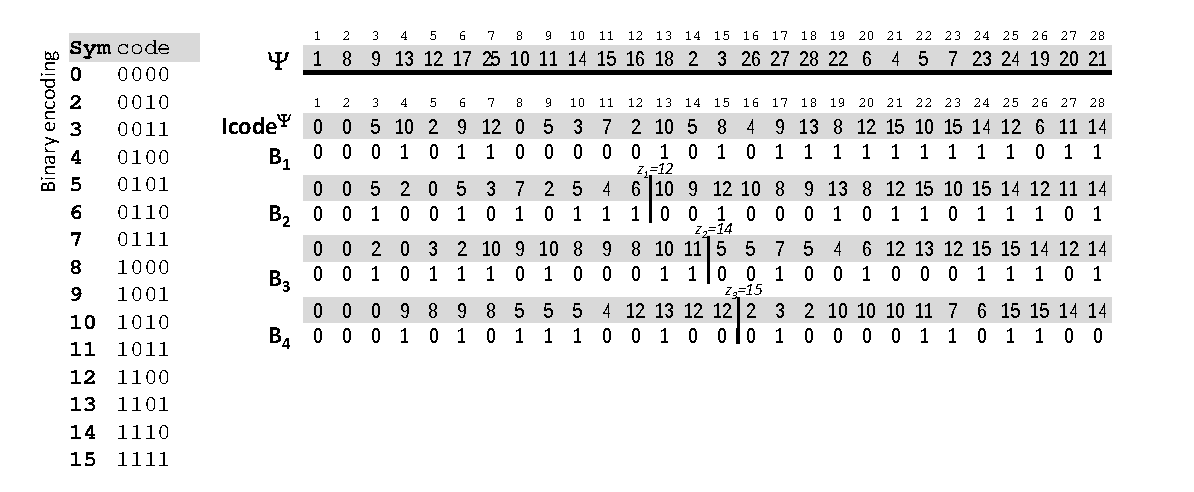
\includegraphics[width=1.0\textwidth]{figures/wma.eps}}
			{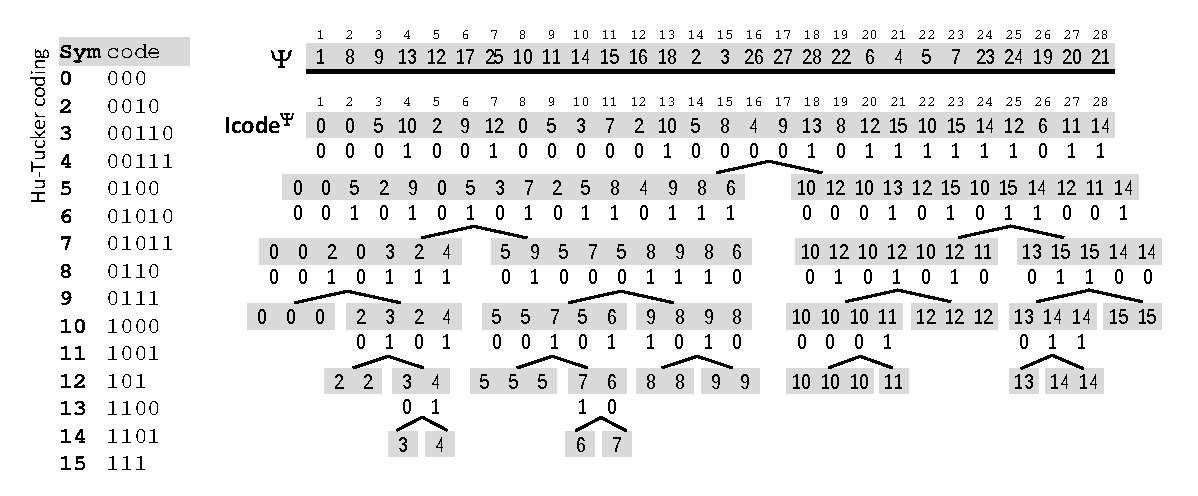
\includegraphics[width=1.0\textwidth]{figures/wta.eps}}
		\end{center}
		\caption{Balanced \acrlong{wm} (top) and \acrlong{htwt} (bottom)}
		\label{fig:wtwm}
	\end{figure}


	In Figure~\ref{fig:wtwm}, we show both the \gls{wm} and the \gls{htwt} built on top of $Icode^{\Psi}$ from Figure~\ref{fig:tcsa}.
	The binary code-assignment to the source symbols $t_i \in I$ and that obtained after applying Hu-Tucker encoding
	algorithm~\cite{hu1971optimal} are also included in the figure.
	
	Since the most useful operation of these two structures for our application, by far, is the $\cnt(i,j,\alpha,\beta)$, we will proceed to explain in detail how the efficiency of that operation has influenced our choice of structures. Just as proven in Section~\ref{sec:wt} with \gls{wt}, both \gls{htwt} and \gls{wm} implement the $\cnt$ operation in $O(\log\sigma)$ time on average. This is easy to prove for \gls{htwt} as each node will contain entries from a lexicographically contiguous subrange from the alphabet $\Sigma$, making the same properties seen for \gls{wt} hold. The main difference is that Hu-Tucker codes will reshape the tree, making the leaves containing the least frequent symbols deeper than the leaves with the more frequent symbols, which may theoretically produce a tree of height $\sigma-1$\footnote{Imagine a vocabulary $\Sigma=\{s_1..s_\sigma\}$, where the probability of appearance of the symbol $s_i$ in the text $S$ turned out to be $2^{-i}$.}, which will obviously affect the worst-case performance, in exchange of a very large compression ratio.

	The complexity may initially seem harder to analyze for \gls{wm}, as its ``nodes'' are delimited implicitly: the symbols with a code starting in 0 will find their second bit in an implicit node delimited by the subrange $B_2[1..z]$ (for some $1 \leq z < n$), while the symbols with a code starting in 1 will correspond to $B_2[z+1..n]$. Generalizing this idea, we can assert that symbols with the same \textit{context} of $\alpha$ starting bits in their codes will find their next $\alpha+1$ bit in some subrange $B_{\alpha+1}[i..j]$ with $1 \leq i \leq j \leq n$. Therefore, the same properties from \gls{wt} can be exploited for a $\cnt$ operation in \gls{wm} as well, allowing us to solve it in $O(\log\sigma)$ worst-case time.

	While it would also be possible to build \gls{wm} using canonical Huffman codes, it is unfortunately impossible guarantee the $O(\log\sigma)$ bound on $\cnt$ on such \gls{wm}, as the symbols lose their original lexicographic proximity, meaning that symbols which would appear on the same node of \gls{wt} due to the common most significant bits in their original codes, would get different Huffman codes based on their frequency of appearance in the text, ending up in separate nodes. On the other hand, to our best knowledge, there is no practical way of building \gls{wm} with Hu-Tucker codes.

	\subsubsection{Implementation details} 
	%We include here details regarding how we tune our \gls{htwt} and \gls{wm}.
	As we discussed in Section~\ref{sec:wt}, both \gls{htwt} and \gls{wm} are built over bitvectors that require support for $\rank$ and $\select$ operations. In our implementations we included two alternative bitvector representations avaliable
	at {\em libcds} library:{\footnote{\url{https://github.com/fclaude/libcds}}}
	
	\begin{itemize}
		\item A plain bitvector based on \cite{Mun96} named {\em RG} with 
		additional structures to support $\rank$ in constant time ($\select$ in logaritmic time).
		{\em RG} includes a sampling parameter ($factor$) that we set to value $32$. In this case,
		our  bitvector {\em RG} uses $n (1+1/32)$ bits. That is, we tune {\em RG} to use a sparse sampling. 
			
		\item A compressed RRR bitvector~\cite{Raman:2002:SID:545381.545411}. The {\em RRR} implementation includes
		a sampling parameter that we tune to values $32$, $64$, and $128$. Higher sampling values achieve better compression.
	\end{itemize}


	In advance, when presenting results for \gls{htwt} and \gls{wm} we will consider the four bitvector configurations
	above. Regarding our implementations of \gls{wm} and \gls{htwt}, note that we reused the same implementation of \gls{wm} from \cite{CNO15}, 
	and we created our custom \gls{htwt} implementation, paying special focus at solving $\cnt$ efficiently.

\section{Algorithms}
	We have X to Y and even Top K queries that are not that hard to describe.

	\subsection{Spatial queries}
	\label{sec:sq}

	With the structure described for representing the spatial component of the trips,
	the following queries can be solved.

	%\vspace{-2mm}
	\begin{itemize}[leftmargin=3mm]
	\setlength{\itemindent}{0mm}
	\item {\em Number of trips starting at node $X$ (\Sswx).}
	Because $\Psi$ was cyclically built in such a way that every $\$$ symbol is followed by the first node 
	of its trip, this query is solved by $[l,r]~\leftarrow~bsearch(\$X)$ over the \gls{csa}, 
	which results on a binary search for the pattern $\$X$ over the section $\Psi[2,z+1]$ corresponding to $\$$ symbols. 
	Then $r-l+1$ gives the number of trips starting at $X$.

	\item {\em Number of trips ending at node $X$ (\Sewx).} In a similar way to the previous query, 
	this one can be answered with $bsearch(X\$)$.

	\item {\em Number of trips starting at $X$ and ending at $Y$ (\Sfxty).}
	Combining both ideas from above, and thanks to the cyclical construction of $\Psi$, this query is solved 
	using $bsearch(Y\$X)$.

	\item {\em Number of trips using node $X$ (\Sux).}
	%Instead of performing a binary search over $\Psi$, we can operate on bitmap $D$. 
	Even though we could solve this query with $bsearch(X)$, it is more efficient to solve it by directly operating on $D$. 
	 Assuming that $X$ is
	at position $p$ in the vocabulary $V$ of  \gls{ctr} ($V[p]=X$), its total frequency is obtained by
	$occs_X \leftarrow select_1(D,p+1) - select_1(D,p)$. %That is, we find the range in $D$ corresponding to the node $X$.
	If $p$ is the last entry in $V$, we set $occs_X \leftarrow n+1-select_1(D,p)$.

	\setlength{\itemindent}{0mm}
	\item {\em Top-k most used nodes (\Stk).}
	We provide two possible solutions for this query named: %These queries have two possible implementations:
	sequential and binary-partition approaches. 

	\begin{itemize}
	\item To return the $k$ most used nodes using {\em sequential approach (\Stkseq)}. The idea is
	to apply  $\select_1$ operation sequentially for every node from $2$ to $|V|$ to compute the 
	frequency of each node and to return the $k$ nodes with highest frequency.
	We use a min-heap that is initialized with
	the first $k$ nodes, and for every node $s$ from $k+1$ to $|V|$, 
	we compare its frequency with that of the minimum node (the root) from
	the heap. In case the frequency of $s$ is higher, the root of the heap is replaced by $s$ and
	then moved down to comply with the heap ordering. At the end of the process, the heap
	will contain the top-k most used nodes $\langle p_1\:,\:p_2,\:\dots,\:p_k \rangle$, which can be 
	sorted with the heapsort algorithm if needed. Finally, we return $\langle V[p_1],V[p_2],\dots,V[p_k]\rangle$.
	Note that this  approach always performs $|V|$ $\select_1$ operations on $D$.

	\item The {\em binary-partition (\Stkbin)} approach takes advantage of a skewed 
	distribution of frequency of the nodes that trips traverse.  Working over $D$ and $V$, we 
	recursively split $D$  into two segments after each iteration. 
	If possible, we leave the same number of different nodes in each side of the partition. 
	Initially, we start considering the range in $D[l,r] \leftarrow D[select_1(D,2),n]=D[z+2,n]$ 
	which corresponds to the nodes that appear in 
	$V$ from positions $i=2$ to $j=|V|$.\footnote{We skip the $\$$ at the first entry of $V$ and its corresponding 
	entries in $D$; that is, $D[1,select_1(D,2)-1]$.}
	%	$D$ (without its initial range 	%of $|V|$ $\$$ symbols).
	We use a priority queue that is initialized as $Q \leftarrow (\langle i,j\rangle, \langle l,r\rangle)$.
	Then, assuming $m=i + \frac{j-i+1}{2}$ and $q=select_1(D,m)$, we create two partitions 
	$D[l, q-1]$ and  $D[q, r]$, which correspond respectively to the nodes in $V[i,m-1]$ and $V[m, j]$.
	These  segments created after the partitioning step are
	pushed into  $Q$. %, storing the initial and the final positions of the segment in $D$,
	%and also the initial and final corresponding positions in $V$. 
	The pseudocode can be found in  Figure~\ref{fig:topk_nieves}.

	The priority of each segment in $Q$ is
	directly the size of its range in $D$ ($r-l+1$). 
	%The priority queue $Q$ is initialized with a segment covering the whole $D$ (without its initial range
	%of $|V|$ $\$$ symbols). 
	When a segment extracted from $Q$ represents the instance of only one node ($(\langle i,j\rangle, \langle l,r\rangle)$, with $i=j$),
	that node is returned as a result of the top-k algorithm (we return $V[i]$). The algorithm stops when the first $k$
	nodes are found.

	For example, when searching for the top-1 most used nodes in the example from Figure~\ref{fig:tcsa}, $Q$ is initialized with
	the segment $[8, 28]$, corresponding to nodes from~1~to~10 (positions from~2~to~11 in $V$). Note
	that the entries of $D$ from~1~to~7 and $V[1]$ represent the $\$$ symbol. Since it is not an actual node, it
	 must be skipped. Then $[8, 28]$ is split producing the segments $[8, 20]$ for nodes 1~to~5 ($V[2,6]$)
	and $[21, 28]$ for nodes~6~to~10 ($V[7,11]$). After three more iterations, we extract
	$(\langle 3,3\rangle, \langle 14,18\rangle)$, hence obtaining the segment $[14, 18]$ for
	the single node 3 (position $4$ in $V$), concluding that the  {\em Top-1 most used node} is 
	$\mathbf{3}=V[4]$ with a frequency equal to $5=18-14$.

	%\marginpar{\tiny algorithm ten que comezar metendo $<2,|V|>$, non $1,V$}
	%\marginpar{\tiny $q$ debe ser $\select_1(D,m)$, non $\select_1(D,m+1)$}


	%	\begin{figure}[t]
	%	%\vspace{-0.5cm}
	%	\begi%n{center}
	%	\begin{minipage}{0.5\textwidth}
	%	\begin{code}
	%	\textbf{GetTopK} $(k)$: \\
	%	 \> $ Q ~\leftarrow$ \textbf{new PriorityQueue()}; \\
	%	 \> $ Q .$\textbf{push$(<1, |V|>, <$\select$_1(D,2), n-1>)$}; \\
	%	 \> $ current\_k ~\leftarrow 0$; \\%\\
	%	
	%	 \> \textbf{while }$current\_k < k$: \\
	%	 \> \> $ (<i,j>, <l,r>) ~\leftarrow ~Q.$\textbf{pop$()$}; \\%\\
	%	
	%	  \> \> \textbf{if} $i = j$: \\
	%	 \> \> \> $ topK[current\_k] ~\leftarrow i$; \\
	%	 \> \> \> $ current\_k ~\leftarrow current\_k + 1$; \\
	%	 \> \> \textbf{else}: \\
	%	 \> \> \> $ m ~\leftarrow i + \frac{j - i + 1}{2}$; \\
	%	 \> \> \> $ q ~\leftarrow$ \textbf{select$_1(D,m + 1)$}; \\
	%	 \> \> \> $ Q .$\textbf{push$(<i, m-1>, <l, q-1>)$}; \\
	%	 \> \> \> $ Q .$\textbf{push$(<m, j>, <q, r>)$}; \\%\\
	%	 %
	%	 \> \textbf{return} $topK$; \\
	%	\end{code}
	%	\end{minipage}
	%	\end{center}
	%	\vspace{-0.2cm}
	%	\caption{Top K most used nodes implementation using binary partitions}
	%	\label{fig:topk_nieves}
	%	%\vspace{-0.5cm}
	%	\end{figure}

	\end{itemize}


	\begin{figure}[t]
		%\vspace{-0.5cm}
		\begin{center}
			\begin{minipage}{0.70\textwidth}
				\begin{code}
					\textbf{GetTopK\_most\_used\_nodes} $(k)$: \\
					\>(l.1~) \> ~$ Q ~\leftarrow$ \textbf{new PriorityQueue()}; \\
					\>(l.2~) \> ~$ Q .$\textbf{push$(\langle2, |V|\rangle, \langle$\select$_1(D,2), n\rangle)$}; \\
					\>(l.3~) \> ~$ current\_k ~\leftarrow 0$; \\%\\
					
					\>(l.4~) \> ~\textbf{while }$current\_k < k$: \\
					\>(l.5~) \> ~\> $ (\langle i,j\rangle, \langle l,r\rangle) ~\leftarrow ~Q.$\textbf{pop$()$}; \\%\\
					
					\>(l.6~) \> ~\> \textbf{if} $i = j$: \\
					\>(l.7~) \> ~\> \> $ topK[current\_k] ~\leftarrow V[i]$; \\
					\>(l.8~) \> ~\> \> $ current\_k ~\leftarrow current\_k + 1$; \\
					\>(l.9~) \> ~\> \textbf{else}: \\
					\>(l.10) \> ~\> \> $ m ~\leftarrow i + \frac{j - i + 1}{2}$; \\
					\>(l.11) \> ~\> \> $ q ~\leftarrow$ \textbf{select$_1(D,m + 1)$}; \\
					\>(l.12) \> ~\> \> $ Q .$\textbf{push$(\langle i, m-1 \rangle, \langle l, q-1 \rangle)$}; \\
					\>(l.13) \> ~\> \> $ Q .$\textbf{push$(\langle m, j \rangle, \langle q, r \rangle)$}; \\%\\
					\>(l.14) \> ~\textbf{return} $topK$; \\
				\end{code}
			\end{minipage}
		\end{center}
		\vspace{-0.3cm}
		\caption{Algorithm {\em Top-k most used nodes} using binary-partition approach.}
		\label{fig:topk_nieves}
		%\vspace{-0.5cm}
	\end{figure}

	\item {\em Top-k most used nodes to start a trip (\Stks).}
	Both \Stk\ approaches above can be adapted for answering \Stks.
	However, unlike its simpler variant, it requires performing $bsearch(\$X)$ over $\Psi$ (rather than a $\select$ on $D$) at
	each iteration, hence increasing the temporal complexity of the operation.

	The implementation of the linear approach is straightforward. The binary-partition approach differs slightly 
	from the algorithm in Figure~\ref{fig:topk_nieves}: in (l.2) we insert $(\langle 2, |V| \rangle, \langle 2,z+1 \rangle)$ into $Q$, and we 
	replace (l.11) with $[x,y]~\leftarrow~bsearch(\$V[m])$; $q \leftarrow x$.

	%interval covers only the range corresponding to $\$$ symbols 
	%(therefore $\langle l,r\rangle \leftarrow \langle 1,z+1\rangle$), and $q$ is computed as $[q,\_]~\leftarrow~bsearch(\$V[m])$.

	%Following the same idea, one could also support querying for the Top-k nodes used to end a trip. 
	\end{itemize}

	\subsection{Temporal queries}
	\label{sec:tq}
	With either one of the described alternatives (\gls{htwt} or \gls{wm}) to represent time intervals
	we can answer the following pure temporal queries:

	\begin{itemize}[leftmargin=3mm]
	\setlength{\itemindent}{0mm}
	%\item {\em Number of nodes used at instant $t$}. This is computed as $\rank_t(n) -rank_t(z+1)$. 
	%That is, to discard the occurrences of $t$ in the $\$$ zone, we count the occurrences of instant $t$ in \gls{wt}, and
	%then we subtract $\rank_t(z+1)$, where $|\mathcal{T}|$ is the number of trips.


	\item {\em Number of trips starting during the time interval $[t_1,t_2]$ (\Tst).} Since we keep the
	starting time of each trip within $Icode^{\Psi}[1,z]$, we can efficiently solve this query 
	by simply computing $\cnt(1,z,t_1,t_2)$.

	\item  {\em Total usage of network stops during the time interval $[t_1,t_2]$ (\Tut).} This query
	can be seem as the sum of the number of trips that traversed each network node during $[t_1,t_2]$.
	We can solve this query by computing $\cnt(z+1,n,t_1,t_2)$. 

	\item {\em Number of trips performed during the time interval $[t_1,t_2]$ (\Ttt).} This is also an
	interesting query that permits to know the actual network usage during a time interval. 
	To solve this query
	we could compute {\em \Ttt} by subtracting the number of trips that started after $t_2$ 
	(\textit{\Tst}$(t_2+1,\sigma^t-1) $) and the number of trips that ended 
	before $t_1$ (\textit{\Tet}$(0,t_1-1) $) from the total number of trips ($z$). 
	However, recall that
	$Icode^{\Psi}[1,z]$ has the starting time of each trip, but we do not keep their ending time.
	We could solve \textit{\Tet}$(0,t_1-1)$ by taking the first node ($X$) of each trip starting
	before $t_1$, then applying $\Psi$ until reaching the ending node ($Y$), and finally getting the ending
	time of that trip associated to node $Y$. However, this would be rather inefficient.
	A possible solution to efficiently solve \textit{\Tet}$(0,t_1-1)$, would require to increment our temporal
	component, in parallel with $Icode^{\Psi}[1,z]$,  with another \gls{wt}-based representation of the 
	ending times for our $z$ trips. This would permit to report the number of trips
	ending before $t_1$ as $\cnt'(1,z,0,t_1-1)$, but would increase the overall size of \gls{ctr}.
	Yet, note that even without keeping ending-times, we could 
	provide rather accurate estimations of \Ttt\ for a system administrator. For example, using \Tut\
	to compute the number of times each trip went through any node during the time interval $[t_1,t_2]$, 
	and dividing that value by the average nodes per trip. Another good estimation can also be obtained with 
	{\em\Tst$(t_1,t_2)$}.


	% 
	% \item {\em Top-k most used times (\Ttk)}. We can follow a similar procedure to that used to solve the {\em Top-k most used
	% 	nodes} discussed in Section~\ref{sec:sq}. We can use both the simpler sequential or a binary-partition approach.
	% For the binary-partition approach we proceed similarly as in Figure~\ref{fig:topk_nieves}. In this case,
	% we start with the root node in the priority queue, and recursively split the
	% extracted node $v$ (whose bitvector is $B_v$) with $n_0 \leftarrow rank_0(B_v,|B_v|)$, 
	% obtaining two new nodes $v_0$ and $v_1$: one for the zeros and another for the ones. The priority of $v_0$ and $v_1$ 
	% depends on the size of the bitmaps in the nodes, for $v_0$ it is $n_0$, whereas for 
	% $v_1$ it is $|B_v| - n_0$. The process stops when the first $k$ leaves are extracted from the queue.
	% 
	% As we will show in Section~\ref{sec:exp:temp}, the binary-partition approach is preferred when the distribution of times 
	% is skewed and the queried $k$ is not large.  Otherwise, the sequential approach is typically preferred.
	\end{itemize}

	\subsection{Spatio-temporal queries}
	\label{sec:stq}
	Apart from the pure spatial and temporal queries discussed in the previous sections, % in Sections~\ref{sec:sq}~and~\ref{sec:tq}, 
	we can combine both the self-indexed spatial and temporal components from \gls{ctr} to answer spatio-temporal queries. 
	The idea is to restrict spatial queries to a time interval $[t_1, t_2]$.  An example of this type of query is to return  the
	{\em number of trips starting at node $X$ that occurred between $t_1$ and $t_2$}, which we can solve by first finding the
	range in the \gls{csa} of the trips starting in $X$ and then relying on the  ${count}$
	operation in the \gls{htwt} (or \gls{wm}). The following spatio-temporal queries can be solved by \gls{ctr}:
	%\marginpar{\tiny ojo, comente operacion ``report''}



	\begin{itemize}[leftmargin=3mm]

		\setlength{\itemindent}{0mm}
		\item {\em Number of trips starting at node $X$ during time interval $[t_1,t_2]$ (\Tswx).}
		Recall that in the time sequence we also included timestamps associated with the area of $\$$-symbols in $\Psi$.
		Particularly, for each $\$$, we keep the time of the first node of its trip. Therefore, 
		we can perform $[l,r]~\leftarrow~bsearch(\$X)$ as in a regular spatial query to find the
		range $\Psi[l,r]$ ($[l,r]\subseteq [2,z+1]$) that corresponds to $\$$ symbols that end a trip
		which started at node $X$. Then, since the time sequence $Icode^{\Psi}$ 
		(represented with either a \gls{htwt} or \gls{wm}) is
		 aligned with $\Psi$, we can filter out those trips that started within $[t_1,t_2]$ performing
		operation $\cnt(l,r,t_1,t_2)$. In Figure~\ref{fig:search2} (steps \textcircled{1} and \textcircled{2}) we can see the steps involved.

	\begin{figure}[thb]
		%\vspace{-0.4cm}
		\begin{center}
			{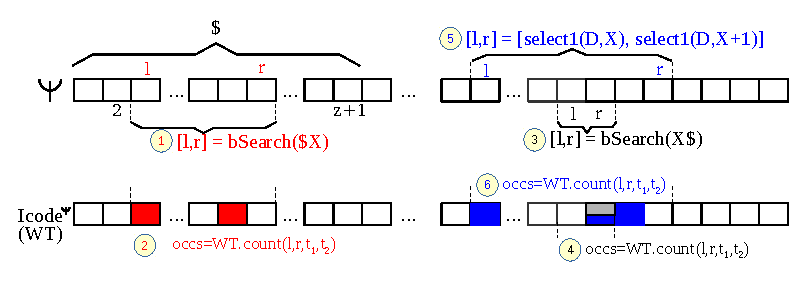
\includegraphics[width=0.90\textwidth]{figures/search2.eps}}
		\end{center}
		\vspace{-0.3cm}
		\caption{Trips staring at, ending at, or using node $X$  during time interval $[t_1,t_2]$.}
		\label{fig:search2}
		%\vspace{-0.6cm}
	\end{figure}
		
		\item {\em Number of trips ending at node $X$ during the time interval $[t_1,t_2]$ (\Tewx). }
		As above, we initially perform the spatial query $[l,r]~\leftarrow~bsearch(X\$)$ to 
		obtain the range in $\Psi$ that corresponds to the pattern $X\$$ (trips ending at node $X$).
		Then, we use  $\cnt(l,r,t_1,t_2)$ operation to count how many of those trips match the temporal constraint.
		See steps \textcircled{3} and \textcircled{4} in Figure~\ref{fig:search2}.
		
		\item {\em Number of trips using node $X$ during the time interval $[t_1,t_2]$ (\Tux).}
		As in the corresponding spatial query, the range $[l,r]$ in $\Psi$  is obtained with two $\select_1$ operations on $D$.
		Finally, $\cnt(l,r,t_1,t_2)$ finds the occurrences within the time interval $[t_1,t_2]$.
		See steps \textcircled{5} and \textcircled{6}  in Figure~\ref{fig:search2}.



	\begin{figure}[thb]
		%\vspace{-0.4cm}
		\begin{center}
			{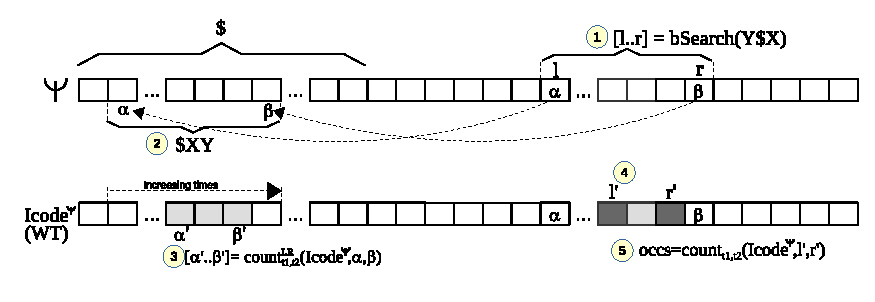
\includegraphics[width=0.90\textwidth]{figures/search.eps}}
		\end{center}
		\vspace{-0.3cm}
		\caption{Trips staring at $X$ and ending at $Y$ during time interval $[t_1,t_2]$.}
		\label{fig:search}
		%\vspace{-0.6cm}
	\end{figure}	
		\item {\em Number of trips starting at $X$ and ending at $Y$ occurring during  time interval $[t_1,t_2]$ (\Tfxty).}
		We consider two different semantics. A query with  {\em strong semantics} will obtain trips
		that start and end within  $[t_1,t_2]$. Whereas, a query with  {\em weak semantics} will obtain trips
		whose time intervals overlap  $[t_1,t_2]$ and, therefore, they could actually start before $t_1$ or end after $t_2$.
		
		In Figure~\ref{fig:search}, we show the step-by-step process to solve this type of queries.
		As in a spatial query, we start by searching for the range $[l,r] \leftarrow bsearch(Y\$X)$ in $\Psi$ corresponding 
		to trips starting at $Y$ and ending at $X$ ({\em step-\textcircled{1}}). Next, due to our sorting of trips,  the range for $Y\$X$ in $\Psi[l,r]$
		can be mapped to a continuous range $[\alpha,\beta]$ of the same size in the $\$XY$ region of $\Psi$. We compute $\alpha \leftarrow \Psi[l], 
		\beta\leftarrow\alpha+r-l$ ({\em step-\textcircled{2}}). Furthermore, note that the range for $\$XY$ preserves the same order as that for $Y\$X$.
		
		At this point, since $Icode^{\Psi}$  was aligned with $\Psi$, 
		we could check ending-time constraints within $Icode^{\Psi}[l,r]$  and starting-time constraints 
		within $Icode^{\Psi}[\alpha,\beta]$ (recall we keep starting times associated with the corresponding $\$$ of each trip).
		Note also that, due to our sorting (by starting-node, ending-node, starting-time,$\dots$) the times in $Icode^{\Psi}[\alpha,\beta]$ are 
		increasing (all of them correspond to trips with the same starting-node $X$ and ending-node $Y$). Therefore,
		we can find the continuous subrange $[\alpha',\beta'] \subseteq [\alpha,\beta] $ corresponding to trips
		that start within $[t_1, t_2]$ ({\em step-\textcircled{3}}). We refer to this operation as $\cntLR$ in Figure~\ref{fig:search}.
		Thus, that assuming $Icode^{\Psi}[\alpha,\beta]$ are increasing,  
		$[\alpha',\beta'] \leftarrow countLR(\alpha,\beta,t_1,t_2)$ would report the 
		positions $[\alpha',\beta'] \subseteq [\alpha,\beta]$ such that $\alpha' = argmin_{x} (Icode^{\Psi}[x] \geq t_1)$ and
		$\beta' = argmax_{x} (Icode^{\Psi}[x] \leq t_2)$.
		
		Using a \gls{wt}, a simple way to implement $\cntLR$  consists in performing  two binary searches within 
		$[\alpha,\beta]$ to find $[\alpha',\beta']$, where at each step we would use $\access$ operation. This would cost $O(\log n \log \sigma)$. 
		Yet, we could also regard on $\cnt$ operation to obtain a more efficient and also rather straightforward 
		implementation of $\cntLR$ so that we set $\alpha' \leftarrow count(\alpha,\beta,-1,t_1-1)$ and
		$\beta' \leftarrow \alpha'+ count(\alpha,\beta,t_1,t_2)$. It costs $O(\log\sigma)$.
		
		
		\begin{itemize}
			\item {\em Strong semantics (\Tfxtys).} Note that the subrange $[\alpha',\beta']$ (containing trips starting within $[t_1,t_2]$) 
			has a matching subrange $[l',r'] \subseteq [l,r]$ ({\em step-\textcircled{4}}), where some of the ending times of these trips will fall inside 
			$[t_1, t_2]$ (this allows us to check the ending time constraint). By performing  $\cnt(l',r',t_1,t_2]$  we get the final result 
			({\em step-\textcircled{5}}). 
			To sum up, answering this query  requires: one $bsearch$ over $\Psi$ (to find $[l,r]$), one $\access$ to $\Psi$ to obtain
			 $\alpha$ ($\beta\leftarrow \alpha+r-l$), one $\cntLR$ to find $[\alpha',\beta']$, and one $\cnt$ 
			 (to count the valid ending times in $[l',r']$).
			
			
			\item {\em Weak semantics (\Tfxtyw).}
			The size of $[\alpha',\beta']$ is already a partial answer. To get the final result, we need to add 
			also the occurrences of those trips starting before $t_1$ that end at $t_1$ or later. 
			To do so, if $l<l'$, we need to compute $\cnt(l,l'-1, t_1, {\sigma_t})$. This gives us the number of time 
			instants in the range $[l,l')$ of  $Icode^{\Psi}$ that fall inside $[t_1, {\sigma_t}]$. 
			That is, ending times equal or after $t_1$.
		\end{itemize}
		
		


	\item {\em Top-k most used nodes during  time interval $[t_1,t_2]$ (\STtk).}
	Both the sequential and binary-partition approaches discussed in Section~\ref{sec:sq} can easily
	be extended to support this query. The idea is that, when we add a node either to the min-heap or priority-queue
	respectively, we compute its frequency within time interval $[t_1,t_2]$ (using $\cnt$ operation) 
	rather than using its overall frequency.

	\begin{itemize}
		\item In the {\em sequential approach (\Stkseq)}, given a node whose corresponding range
		in $\Psi$ is $D[l,r]$, we compute its frequency using $\cnt(l,r,t_1,t_2)$ instead of simply using  $r-l+1$. 
		The rest of the process is exactly as discussed for the pure spatial \Stkseq\ query.
		
		\item In the {\em binary-partition approach (\Stkbin)}, we have to consider the priority of a
		given segment as the number of trips covered by that segment that occurred during $[t_1,t_2]$. Again, given
		a segment $[l,r]$ in $\Psi$ we compute that priority as $p_l^r \leftarrow count(l,r,t_1,t_2)$ instead of 
		$p_l^r \leftarrow  r-l+1$. Apart from
		that, the only modifications that we must consider over the pure spatial \Stkbin\ algorithm in 
		Figure~\ref{fig:topk_nieves} are:
		we replace (l.2) by $p_l^r \leftarrow count(select_1(D,2),n,t_1,t_2)$; $Q.push(\langle2, |V|\rangle, \langle select_1(D,2), n\rangle, \underline{p_l^r})$,
		and we replace  (l.12) and (l.13) respectively by 
		   $ Q.push(\langle i, m-1 \rangle, \langle l, q-1 \rangle, \underline{count(l,q-1,t_1,t_2)})$ and
		   $ Q.push(\langle m,   j \rangle, \langle q,   r \rangle, \underline{count(q,r,t_1,t_2)})$.
		
	\end{itemize}


	\item {\em Top-k most used nodes to start a trip during time interval $[t_1,t_2]$(\STtks).}
	Following the same guidelines discussed above for \STtk, adapting the  sequential and 
	binary-partition solutions for the spatial \Stks\ to include temporal constraints is straightforward.	
		
		
	\end{itemize}


\section{Experiments}
	We may have not compared it to anything but we sure do have tons of results!

	We have run experiments to evaluate both the space requirement and performance at query time of \gls{ctr}
	when dealing with spatial, temporal and spatio-temporal queries over two different datasets 
	(Porto and Madrid) that are described in Section~\ref{sec:ed}. 

	We have used several configurations of \gls{ctr} by tuning both its
	spatial and temporal components. In the spatial part, %(Section~\ref{sec:transnet_repr}), 
	we set the  $\Psi$ sampling parameter ($t_{\Psi}$) to the values $t_{\Psi} = \{32, 128, 512\}$. 
	For the temporal component, % (Section~\ref{sec:time_repr}), 
	we have tested both the 
	balanced \gls{wm}, and the Hu-Tucker-shaped \gls{wt} (\gls{htwt}) using the same bitvector configurations
	discussed in Section~\ref{sec:time_exp}. That is, using either a plain bitvector $RG$ with a 
	sparse sampling ($RG_{32}$), or a $RRR$ bitvector with sampling parameter $\in \{32,64,128\}$ 
	($RRR_{32}, RRR_{64}$, and $ RRR_{128})$.


	\subsection{Experimental datasets}
	\label{sec:ed}
	We used two different datasets of trips in our experiments:
	\begin{itemize}
	   %%%%%%%%%	
	  \item {\bf Madrid dataset}:
	  Using GTFS\footnote{GTFS is a well-known specification for representing an urban transportation network. See
	  \url{https://developers.google.com/transit/gtfs/reference?hl=en}} data from the  public transportation network of 
	  {Madrid},\footnote{Data from
	  the EMT corporation at \url{https://www.emtmadrid.es/movilidad20/googlet.html}} we generated a dataset of 
	  synthetic trips combining the subway network with the Spanish commuter rail system (called {\em cercanías}).
	  In total, there are $313$ different stations/nodes from $23$ lines.
	 
	We generated $10$ million trips with lengths varying from $2$ to $31$ nodes traversed. Those lengths follow a binomial 
	distribution. The average length of the trips is $11.81$ nodes. 
	%
	%	\marginpar{\tiny \OJOFARI{Daniil, se hace asi realmente? porfa check}}
	%	In the generation of a trip of length $l$, we randomly choose a starting node from a line and the starting direction. Then, we follow that line until 
	%	we reach a switching node. At this node, we choose the line and direction to follow with uniform distribution. We avoid repeated nodes in the trip.
	%	Generation ends when $l$ nodes have been added to the trip.

	In the generation of a trip of length $l$, we randomly choose a starting node from a line, and the starting direction. 
	Then, we follow that line until we reach a switching node. At this node, we decide whether to follow the current 
	line or to switch to a new line. We allow only up to four line switches for a given trip, and use fixed probability 
	values to decide whether to switch line or not. Such probability is $0.5$, $0.1$, $0.05$, and $0.02$ respectively 
	for the first, second, third, and fourth line switch in a trip. 
	We also avoid revisiting nodes in the same trip. 
	Generation process ends when $l$ nodes have been added to the trip, or a dead end is reached.

	As a baseline, the plain representation of the generated trips using a $9$-bit integer ($\lceil\log_2 314\rceil= 9$) 
	for every node-ID (and $\$$ separator) would require $137.47$ MiB.

	 
	%We also generated synthetic times for those trips that can be seen in Figure~\ref{fig:distrib} with the label 
	%\textit{skewed}, so most of the trip timestamps belong to rush hours. 
	We also generated synthetic times for those trips following the same rules used to create the time distribution
	named \textit{skewed} in Figure~\ref{fig:distrib}, so most of the trip timestamps belong to rush hours. 
	Yet, instead of using only regular working days, we distinguished four kinds of days in a week: 
	regular working days; Fridays and holiday eves; Saturdays; and Sundays and holidays. We also 
	assume that there are two kinds of weeks related to high and low season periods. 
	Therefore, a time interval may belong to eight types of day. 
	When discretized at five-minute intervals we obtain $2,\!304$ distinct time intervals, 
	while when we use thirty-minute intervals we obtain $384$. In the former case, our  baseline
	 for the generated times using  $12$ bits per time-ID would occupy $183.30$ MiB. In the latter one, each
	time-ID requires  $9$ bits and the  temporal baseline requires $137.47$ MiB.

	%
	%\marginpar{\tiny OJO Tal y como se generan las probabilidades de tiempos para cada tiempo, sólo estamos considerando un tipo de tiempo}
	%

	   %%%%%%%%%
	   \item \textbf{Porto dataset}:
		We downloaded a collection of $1,\!710,\!671 $ trajectories from the city of {Porto} corresponding to taxi trips during 
		a full year (from July 1, 2013 to June 30, 2014), provided by \cite{moreira2013predicting}.\footnote{Description at \url{http://www.geolink.pt/ecmlpkdd2015-challenge/dataset.html}. Download at \url{https://archive.ics.uci.edu/ml/machine-learning-databases/00339/train.csv.zip}} Among other
		fields those data include, for each taxi ride, a list of GPS coordinates and times gathered every $15$ seconds of
		the trip. We adapted such data to our needs by using a map matching algorithm provided by the Graphhopper library,\footnote{\url{https://github.com/graphhopper/map-matching}}
		 and OpenStreetMap cartography.\footnote{\url{http://www.openstreetmap.org/}} This permitted us to
	  figure out the streets that trips were passing through. Finally, trips were encoded as a sequence of identifiers
	  corresponding to adjacent stretches of street (that is, basic street segments with no intersections) the trip traversed, 
	  each one of them tagged with a timestamp.

	  %[1] https://archive.ics.uci.edu/ml/machine-learning-databases/00339/train.csv.zip
	  %[2] https://archive.ics.uci.edu/ml/datasets/Taxi+Service+Trajectory+-+Prediction+Challenge,+ECML+PKDD+2015
	  
	  After filtering incomplete matches, $1,\!617,\!774$ trips, built  over $59,\!618$ distinct street segments, were used for the dataset. 
	  Due to the nature of the network and the trips, 
	  %the average length per trip is longer than in Madrid, of $64.74$ street segments. 
	  the average number of street segments per trip is $64.74$; that is, the length of the trips is longer than in Madrid dataset.
	  Since we needed $16=\lceil\log_2 59,\!618 \rceil$ bits to represent each segment in a trip, the total size of our
	  plain spatial baseline is $202.85$ MiB.

	  For the temporal part, we considered only one kind of day. Therefore, when we sample those $24$ hours into five-minute intervals,
	  we obtain $288$ distinct time intervals that are given a $9$-bit time-ID. Consequently the overall size of the temporal
	  baseline becomes $114.10$ MiB. However, if we split those $24$ hours into thirty-minute intervals, only $48$ time intervals 
	  arise. In this case, each time-ID needs only $6$ bits and the total size of the temporal baseline is $76.07$ MiB.
	\end{itemize}



	\subsection{Space Requirements of \acrshort{ctr}}\label{sec:exp.space}
	We show the compression obtained by \gls{ctr} when built on our two test datasets. Compression is shown
	as the percentage of the size of the plain baselines discussed above.
	Using different configurations of \gls{ctr}, we will show the compression of the spatial component (\gls{csa}), 
	that of the temporal component (\gls{htwt} and \gls{wm}), and finally the overall compression of \gls{ctr}.


	\begin{table}[htb]
	%\vspace{-6mm}
	\begin{center}
	\scriptsize
	  \begin{tabular}{|l|*{3}{r}|}
	  \cline{2-4}
	  \multicolumn{1}{c|}{} & \multicolumn{3}{c|}{$t_{\Psi}$ } \\
	  \multicolumn{1}{c|}{} & 32 & 128 & 512 \\
	  \hline
	  Madrid & 41.32\% & 26.80\% & 23.06\% \\
	  Porto & 23.66\% & 15.49\% & 13.37\% \\
	  \hline
	  \end{tabular}
	%\vspace{-5mm}
	%\caption{Compression of the spatial component with respect to the spatial-only baseline.}
	\caption{Compression of \acrlong{csa} with respect to the spatial baseline.}
	\label{table:spatial_spaces}
	\vspace{-3mm}
	\end{center}
	\end{table}

	Results regarding the compression obtained by \gls{csa} are given in Table~\ref{table:spatial_spaces}.
	The compression ratio is calculated over a plain spatial-only (stop-IDs or street-segment-IDs in each case) representation.   %\marginpar{\tiny Daniil, incluyes separadores aqui ?}
	%Note that an $\icsa$  built on English text~\cite{FBNCPR12} typically
	%reached the compression of {\em gzip} (around 35\% in compression ratio).
	%As expected, the high compressibility of our sorted datasets of trips permits \gls{csa} to improve 
	%those numbers with compression ratios under 30\% in the most sparse setup, while also offering indexing features 
	%that allow us to perform efficient searches.
	In a rather dense 
	configuration of \gls{csa} with $t_{\Psi}=32$ we obtain compression ratios around $41$\% and $23$\% for Madrid and Porto datasets respectively.
	Those results are interesting from the simple point that the baseline representations were only using respectively 
	$9$-bits per node (Madrid) and $16$-bits per segment (Porto). 
	As expected, compression improves as we increase the $\Psi$ sampling parameter $t_{\Psi}$. We show that by tuning 
	\gls{csa} in a more sparse setup we can almost halve the space needs of using $t_{\Psi}=32$. Yet, the resulting \gls{csa} would become
	much slower as we will see in the next section.
	In general, we can see that \gls{csa} obtains better compression in Porto than in Madrid. This is probably due to the longer and
	more predictable trips. Note that is not common to arrive at an intersection having more than two valid 
	street links where to navigate to.


	\begin{table}[htb]
	%\vspace{-6mm}
	\begin{center}
	\scriptsize
	\setlength\tabcolsep{2pt}
	  \begin{tabular}{|l|*{4}{r}|}
	  \cline{2-5}
	  \multicolumn{1}{c|}{} & \multicolumn{4}{c|}{Type of bitvector in \gls{wm}/\gls{htwt}}\\

	  \multicolumn{1}{c|}{}   & $RG_{32}$& $RRR_{32}$& $RRR_{64}$& $RRR_{128}$\\
	  \hline                                             
	  Madrid (\gls{htwt}, 5-min) &  91.33\% &	 80.89\% &	 76.90\% & 	 74.90\% \\
	  Madrid (\gls{wm}, 5-min)   & 103.13\% &	 86.03\% &	 80.61\% & 	 77.88\% \\
	  Madrid (\gls{htwt}, 30-min)&  92.30\% &	 78.90\% &	 74.66\% &	 72.52\% \\
	  Madrid (\gls{wm}, 30-min)  & 103.14\% &	 83.32\% &	 77.90\% &	 75.18\% \\
	  \hline                  
	  Porto (\gls{htwt}, 5-min)  &  93.52\% &	102.61\% &	 98.27\% &	 96.11\% \\
	  Porto (\gls{wm}, 5-min)    & 103.13\% &	106.88\% &	101.41\% &	 98.66\% \\
	  Porto (\gls{htwt}, 30-min) &  96.00\% &	103.78\% &	 99.08\% &	 96.74\% \\
	  Porto (\gls{wm}, 30-min)   & 103.12\% &	107.00\% &	101.50\% &	 98.75\% \\

	  \hline
	  \cline{2-5}
	  \end{tabular}
	%\vspace{-1mm}
	\caption{Compression of \acrlong{wm} and \acrlong{htwt} with respect to the temporal baseline.}
	\label{table:ctr_wt_spaces}
	\vspace{-3mm}
	\end{center}
	\end{table}



	In Table~\ref{table:ctr_wt_spaces}, we focus on the space needed by the temporal component of \gls{ctr}. 
	In this case we show the compression ratios obtained by \gls{htwt} and \gls{wm} %(our two alternative representations) 
	considering that time is either discretized into $5$-min or $30$-min intervals. Recall that the size of the 
	plain baseline representations differs depending on the discretization period. Both \gls{htwt} and \gls{wm} were tuned by
	using bitvector representations $RG_{32}$, $RRR_{32}$, $RRR_{64}$, and $ RRR_{128}$.

	It is interesting to see that in the synthetic dataset from Madrid $RRR$ bitvectors always lead to a better 
	compression than the plain $RG$, while in the real dataset from Porto that is never the case. 
	In some cases the $RRR$ does not compress the times at all. Consequently, for Porto dataset, the faster plain $RG$ 
	bitvectors are probably the best choice. In Madrid dataset, we can see an actual space/time trade-off: $RRR$ obtains better
	compression but will be slower (as we will see in the next section).



	\begin{table}[ht!]
	%\vspace{-6mm}
	\begin{center}
	\scriptsize
	\setlength\tabcolsep{2pt}
	  \begin{tabular}{|l|*{4}{c}|*{4}{c}|}
	  \cline{2-9}
	  \multicolumn{1}{c|}{} & \multicolumn{4}{c|}{Type of bitvector in \gls{wm}/\gls{htwt}}& \multicolumn{4}{c|}{Type of bitvector in \gls{wm}/\gls{htwt}} \\

	  \multicolumn{1}{c|}{}     &$RG_{32}$& $RRR_{32}$& $RRR_{64}$&$RRR_{128}$&$RG_{32}$& $RRR_{32}$& $RRR_{64}$&$RRR_{128}$ \\
	  \hline                                             
	  Madrid (\gls{htwt}, 5-min)  & 69.90\% &   63.93\% &   61.65\% &   60.51\% & 62.07\% &	56.10\% &	53.82\% &	 52.68\% \\
	  Madrid (\gls{wm}, 5-min)     & 76.64\% &   66.87\% &   63.77\% &   62.21\% & 68.81\% &	59.04\% &	55.94\% &	 54.38\% \\
	  Madrid (\gls{htwt}, 30-min) & 66.81\% &   60.11\% &   57.99\% &   56.92\% & 57.68\% &	50.98\% &	48.86\% &	 47.79\% \\
	  Madrid (\gls{wm}, 30-min)    & 72.23\% &   62.32\% &   59.61\% &   58.25\% & 63.10\% &	53.19\% &	50.48\% &	 49.12\% \\
	  \hline
	  Porto (\gls{htwt}, 5-min)   & 48.81\% &   52.08\% &   50.52\% &   49.74\% & 42.22\% &	45.49\% &	43.93\% &	 43.15\% \\
	  Porto (\gls{wm}, 5-min)      & 52.27\% &   53.62\% &   51.65\% &   50.66\% & 45.68\% &	47.03\% &	45.06\% &	 44.07\% \\
	  Porto (\gls{htwt}, 30-min)  & 43.39\% &   45.51\% &   44.23\% &   43.59\% & 35.91\% &	38.03\% &	36.75\% &	 36.11\% \\
	  Porto (\gls{wm}, 30-min)     & 45.33\% &   46.39\% &   44.89\% &   44.14\% & 37.85\% &	38.91\% &	37.41\% &	 36.66\% \\
	  \hline
	  \cline{2-9}
	  \multicolumn{1}{c|}{} & \multicolumn{4}{c|}{$t_{\Psi}=32$}& \multicolumn{4}{c|}{$t_{\Psi}=512$} \\
		\cline{2-9}
	  \end{tabular}
	%\vspace{-5mm}
	\caption{Overall compression of \acrshort{ctr} including different configurations for both the spatial and temporal components.  }
	\label{table:ctr_spaces}
	\vspace{-4mm}
	\end{center}
	\end{table}


	Finally, in Table~\ref{table:ctr_spaces}, we show the overall compression ratios of  \gls{ctr}.
	We use the same configurations for \gls{htwt} and \gls{wm}  as in Table~\ref{table:ctr_wt_spaces}, and both the
	most dense and sparse tuning of \gls{csa} ($t_{\Psi}= 32$ and $t_{\Psi}= 512$ respectively).
	For Madrid dataset, the pair (node,timestamp) is represented with $9+9=18$ bits in our baseline representation 
	when time is discretized into $30$-minute intervals, and with $9+12=21$ when we use $5$-minute intervals.
	In the case of Porto dataset, when using $30$-minute intervals, each pair (node,timestamp) from the baseline requires $16+9=25$ bits. 
	If discretization considers $5$-minute intervals, the baseline requires $16+6=22$ bits. We can see that the overall
	compression of \gls{ctr} in Madrid dataset ranges between $76\%$ and $50\%$. Also we show that Porto dataset is much
	more compressible, obtaining compression ratios from around $50\%$ to $35\%$.


	% \begin{table}[h!]
	% %\vspace{-6mm}
	% \begin{center}
	% \scriptsize
	%   \begin{tabular}{|l|l|c|*{4}{c}|*{4}{c}|}
	%   \cline{3-11}
	%   \multicolumn{2}{l|}{} & \multicolumn{9}{c|}{Times representation} \\
	%   \cline{3-11}
	%   \multicolumn{2}{l|}{} & None & \multicolumn{4}{|c|}{Hu-Tucker Wavelet Tree} & \multicolumn{4}{c|}{Wavelet Matrix} \\
	%   \cline{3-11}
	%   \multicolumn{2}{l|}{} & & RG32 & RRR32 & RRR64 & RRR128 & RG32 & RRR32 & RRR64 & RRR128 \\ \hline
	%   \multirow{4}{*}{\rotatebox{90}{$\Psi_{sampling}$}} & None & & 103.13\% & 86.03\% & 80.60\% & 77.88\% & RG32 & RRR32 & RRR64 & RRR128 \\ %\hline
	%   & 32 & 41.32\% & RG32 & RRR32 & RRR64 & RRR128 & RG32 & RRR32 & RRR64 & RRR128 \\ %\hline
	%   & 128 & 26.80\% & RG32 & RRR32 & RRR64 & RRR128 & RG32 & RRR32 & RRR64 & RRR128 \\ %\hline
	%   & 512 & 23.06\% & RG32 & RRR32 & RRR64 & RRR128 & RG32 & RRR32 & RRR64 & RRR128 \\ \hline
	%   \end{tabular}

	%   \begin{tabular}{|l|*{5}{c}|}
	%   \hline
	%   \diagbox{$\Psi_{sampling}$}{bitmap} & None & RG32 & RRR32 & RRR64 & RRR128 \\ \hline
	%   None & & RG32 & RRR32 & RRR64 & RRR128 \\ %\hline
	%   32 & 56.81 & RG32 & RRR32 & RRR64 & RRR128 \\ %\hline
	%   128 & 36.85 & RG32 & RRR32 & RRR64 & RRR128 \\ %\hline
	%   512 & 31.71 & RG32 & RRR32 & RRR64 & RRR128 \\ \hline
	%   \end{tabular}
	% %\vspace{-5mm}
	% \caption{Test table}
	% \label{table:madrid_spaces}
	% %\vspace{-10mm}
	% \end{center}
	% \end{table}



	%%%%%%%%%%% DESCOMENTAR CUANDO FARI CAMBIE DE OPINION %%%%%%%%%%%

	% \begin{table}[h!]
	% %\vspace{-6mm}
	% \begin{center}
	% \scriptsize
	%   \begin{tabular}{l*{4}{c}|*{4}{c}|r|}
	%   %\hline
	%   & \multicolumn{4}{c}{Hu-Tucker \gls{wt}} & \multicolumn{4}{c}{\gls{wm}} & \multicolumn{1}{r}{} \\
	%   \cline{2-9}
	%   & RG32 & RRR32 & RRR64 & RRR128 & RG32 & RRR32 & RRR64 & \multicolumn{1}{c}{RRR128} & \multicolumn{1}{r}{} \\ \hline

	%   X To Y (s) & RG32 & RRR32 & RRR64 & RRR128 & RG32 & RRR32 & RRR64 & RRR128 & \multirow{7}{*}{\rotatebox{270}{5 minutes}} \\
	%   X To Y (s) & RG32 & RRR32 & RRR64 & RRR128 & RG32 & RRR32 & RRR64 & RRR128 & \\
	%   X To Y (s) & RG32 & RRR32 & RRR64 & RRR128 & RG32 & RRR32 & RRR64 & RRR128 & \\
	%   X To Y (s) & RG32 & RRR32 & RRR64 & RRR128 & RG32 & RRR32 & RRR64 & RRR128 & \\
	%   X To Y (s) & RG32 & RRR32 & RRR64 & RRR128 & RG32 & RRR32 & RRR64 & RRR128 & \\
	%   X To Y (s) & RG32 & RRR32 & RRR64 & RRR128 & RG32 & RRR32 & RRR64 & RRR128 & \\
	%   Starts In X & RG32 & RRR32 & RRR64 & RRR128 & RG32 & RRR32 & RRR64 & RRR128 & \\ \hline

	%   \end{tabular}
	% %\vspace{-5mm}
	% \caption{Test table}
	% \label{table:madrid}
	% %\vspace{-10mm}
	% \end{center}
	% \end{table}



	%%%%%%%%%%%%%%%%%%%%%%%%%%%%%%%%%%%%%%%%%%%%%%%%%%%%%%%%%%%%%%%%%%%%%%%%%%%%%%%%%%%%%%%%%%%%%%%%
	%%%%%%%%%%%%%%%%%%%%%%%%%%%%%%%%%%%%%%%%%%%%%%%%%%%%%%%%%%%%%%%%%%%%%%%%%%%%%%%%%%%%%%%%%%%%%%%%

	\subsection{Performance at query time}
	Through this section, we evaluate the time performance of \gls{ctr} when solving spatial, temporal, and spatio-temporal queries.
	We have randomly generated $10,\!000$ query patterns from our two datasets for each type of query.
	Each time measurement presented below is the average execution time of $10,\!000$ runs using the corresponding query patterns, 
	except for the \Stk\ queries where we perform $100$ runs of the {\em top-k} algorithms with $k=\{10,100\}$.

	Our test machine has an Intel(R) Core(tm) i5-4690@3.50GHz CPU (4 cores/4 siblings) and 8GB of DDR3 RAM. 
	It runs Ubuntu Linux 16.04 (Kernel 4.4.0-21-generic). The compiler used was g++ version 5.4.0 and we set compiler optimization flags to $-O9$. All our experiments run in a single core and time measures refer to CPU user-time.

	During the generation of query patterns, for those queries involving only one node $X$ from the network, 
	we have randomly chosen $X$ $10,\!000$ times from the available network nodes. 
	This is the case of the query patters used both for
	the spatial queries \Sswx, \Sewx, and \Sux\ or the spatio-temporal \Tswx, \Tewx, and \Tux.
	In the case of the spatial \Sfxty\ and the spatio-temporal \Tfxtys, and \Tfxtyw\ the pair of
	network nodes $\langle X,Y \rangle$ that compose our
	query patterns were generated by randomly choosing
	$10,\!000$ trips and then extracting the initial $X$ and ending $Y$ nodes of those trips.

	Moreover, we also generated the time intervals $[t_1,t_2]$ required for 
	the spatio-temporal queries. Considering the different available time-IDs, we chose a random starting
	instant $t_1$ and then randomly generated the width of that interval from five minutes to two hours.
	Note that if we discretized time into $5$-minute intervals and $interval$-$width=59$ minutes, our time
	interval $[t_1,t_2]$ would contain exactly $12$ time IDs ($t_2\leftarrow t_1+11$). However, if time was
	discretized into $30$-minute intervals, $[t_1,t_2]$ would contain only $2$ time IDs ($t_2\leftarrow t_1+1$).
	We followed the same procedure to gather the query patterns used for the pure temporal queries \Tut\ and \Tst.
	%queries \Tuti\ and \Tutr. 
	%Yet, since \Tuti\ only needs a unique time-ID, we only randomly extracted $t_1$.


	%Each time result was the average of the execution of 10000 random queries of that type, except for the top-k queries. 
	%The time intervals for the spatio-temporal queries were generated with a random size from five minutes to two hours.

	%\OJOFARIDONE{posiblemente no tabla con todas las queries, pq -las probamos todas-}

	\subsubsection{Space/time trade-off when dealing with spatial queries} \label{sec:exp:temp}

	In Figures~\ref{fig:madridsp} and \ref{fig:portosp}, we show the performance of \gls{ctr} at
	solving spatial queries for Madrid and Porto datasets respectively. 
	Note that all these queries can be answered using only the \gls{csa} component
	of \gls{ctr}. Therefore, the size of the temporal component 
	is not considered here and compression values (x-axis) refer only to the size of \gls{csa} with
	respect to the spatial baseline as in Table~\ref{table:spatial_spaces}. 
	We show the average query time (in $\mu$s) depending on the
	space used by \gls{csa} with three different 
	sampling configurations ($t_{\Psi} =\{512, 128, 32\}$).


	%It is worth noting 
	Results show that the queries that involve searching in the $\$$ region of 
	$\Psi$, such as \Sswx\ or \Sfxty\ are considerably slower than queries \Sewx\ and \Sux\ 
	due to the large size of that region. Recall there is one $\$$ for every trip. 
	%
	%This difference is much more accentuated if a forward search was used in the \gls{csa}.

	%\marginpar{\tiny Daniil, como se implementa backward search? supongo que usas select para localizar zona para X y luego bsearch dentro de esa %zona? Ya me comentaras...}  Ok, correcto! ;)


	%%%%%%%%%%% MADRID -SPATIAL %%%%%%%%%%%%%
	\begin{figure}[htb]
		%\vspace{-0.4cm}
		\begin{center}
			{\includegraphics[angle=-90,width=0.45\textwidth]{figures_synt/madrid_spatial.eps}}
			{\includegraphics[angle=-90,width=0.45\textwidth]{figures_synt/madrid_spatial_topk.eps}}
		\end{center}
		\vspace{-0.3cm}
		\caption{Spatial queries (left) and spatial {\em top-k} queries (right) for Madrid.}
		\label{fig:madridsp}
		\vspace{-0.3cm}
	%\end{figure}




	%%%%%%%%%%% PORTO - SPATIAL %%%%%%%%%%%%%
	%\begin{figure}[htb]
		%\vspace{-0.4cm}
		\begin{center}
			{\includegraphics[angle=-90,width=0.45\textwidth]{figures_synt/porto_spatial.eps}}
			{\includegraphics[angle=-90,width=0.45\textwidth]{figures_synt/porto_spatial_topk.eps}}
		\end{center}
		\vspace{-0.3cm}
		\caption{Spatial queries (left) and spatial {\em top-k} queries (right) for Porto.}
		\label{fig:portosp}
		%\vspace{-0.6cm}
	\end{figure}

	In both datasets, we can see that \Sux\ (solved using {\em select} on $D$ rather than
	$bsearch$ on $\Psi$) is the fastest query. On average, it takes only around $10$ns
	per query. Except in the most sparse configuration of \gls{csa}, queries \Sewx, \Sswx, and 
	\Sfxty\ require typically less than $10\mu$s. This basically shows the cost of performing
	$bsearch$ on a compressed $\Psi$. In the most sparse setup, times for \Sswx\ and \Sfxty\ are always better 
	in Madrid than in Porto dataset, and \Sewx\ draws rather identical times.
	With the densest configuration  ($t_{\Psi}=32$), \Sewx\ and \Sfxty\ are respectively 
	around $10$-$20$\% fastest in Madrid dataset (\Sewx\ takes $4.05\mu$s and $4.51\mu$s respectively, and
	\Sfxty\ takes $4.54\mu$s and $5.66\mu$s). However, \Sswx\ performs around $20$\% faster in Porto dataset 
	($2.28\mu$s vs $2.90\mu$s).
	\medskip

	%Ends-with-X   Madrid/Porto (4.05/4.51)
	%F-X-to-Y     Madrid/Porto (4.54/5.66)
	%Starts-with-X   Madrid/Porto (2.90/2.28)

	%Regarding \Stk\ queries we can see that the fact of having less trips, but a larger vocabulary, make
	%\Stk\ queries to perform slower at Porto than at Madrid dataset.

	Focusing on \Stk\ queries, we can see huge differences between \Stks\  
	and the rest of the \Stk\ queries, as the former needs to perform {$ bsearch$} over the compressed $\Psi$
	instead of a $\select$ on $D$. 

	We can also see that due to the small number of stops in Madrid dataset, it is always more efficient 
	to use the sequential version of \Stks\ and \Stk\ algorithms. This is also because a rather uniform frequency among nodes 
	increases the number of insertions in the priority queue ($i$) of the binary algorithm
	needed for retrieving the first $k$ nodes ($i \approx |V|$). Moreover, note that for the sequential algorithm 
	$i$ is  at most $|V|$, whereas for the binary-partition counterpart it could become up to $2|V|-1$.


	However, in Porto dataset, where nodes follow a biased distribution (some streets are far more used than others
	by taxis), and whose vocabulary 
	is $190$ times larger than that of Madrid's, the binary-partition version of \Stks\ and \Stk\ algorithms is clearly
	faster than the sequential counterpart (\Stkseq\ and \Stksseq).
	Note that in Madrid dataset, \Stcien\ returns 32\% of the nodes (hence sequential processing worths it) 
	whereas in Porto dataset less than 0.2\% of the nodes are returned. 

	The gap between \Stdiezseq\ and \Stcienseq\ that we can clearly appreciate in Madrid dataset 
	is due to the cost of the insertion of nodes in the min-heap. However, the gap between 
	the binary \Stdiez\ and \Stcien\ 
	is mainly related to the number of iterations performed until the binary-partition algorithm gathers the first
	$10$ and $100$ {nodes}  returned respectively. The same discussion applies for \Stks\ queries.

	%\begin{itemize}
	%	\item top-100-starts en Madrid: seq y bin son similares en tiempo: solo hay 314 nodos en la red y 
	%	top-100starts devuelve el 33\% de los nodos. En Porto, top-100-starts devuelve el 0.2\% de los nodos 
	%	de la red por ello bin es mucho mejor opcion que seq.
	%	\item top-10-starts
	%\end{itemize}





	%We evaluated \gls{ctr} over the Porto dataset, with the same index configurations and type of queries as for Madrid. 
	%Figure~\ref{fig:portosp} shows the performance of the spatial component. It is significantly slower than with Madrid 
	%in the sparse configuration for the \texttt{starts-with-x} or \texttt{from-x-to-y}.

	%\OJOFARI{DANIIL dice aqui que la siguiente frase no es valida: en concreto me dice que: esa frae la puse para explicar
	% starts-with-x y from-x-to-y, pero estoy viendo que no es valida para explicar form-x-to-y. Asi que no se porque  
	% from-x-to-y es mas lenta en un lado que en el otro (Madrid vs Porto)} 
	%This is because the generated queries are with random street segment identifiers, while most of them have never been 
	%used as a starting stop for a taxi, thus triggering the worst case of a binary search.

	%We can also see that because of the increased size of the vocabulary, the sequential versions of top-k perform much 
	%slower than their binary counterparts.


	\subsubsection{Comparing the space/time trade-off of WM and HTWT}
	\label{sec:time_exp}
	In order to compare the efficiency of our \gls{htwt} (that uses variable-length codes and supports $\cnt$ efficiently)
	 with a balanced \gls{wm} alternative under 
	different time distributions (recall that this \gls{wm} is time distribution invariant), 
	we run some experiments that evaluate the average time to execute $\cnt$ operation on
	both representations.

	\begin{figure}[tbp]
		\begin{center}
			\includegraphics[angle=-90,width=0.75\textwidth]{figures_synt/timedistrib.eps}		
			\caption{Time distributions used. The y-axis indicates the number of passengers per each 5-min interval.}
			\label{fig:distrib}
		\end{center}
		\vspace{-3mm}
	\end{figure}

	We used a dataset of generated trips  (Refer to Section~\ref{sec:ed} for the details about Madrid dataset) and we
	generated three kinds of time distributions for our evaluation. We refer to them as: uniform, skewed and very skewed. They are shown
	in Figure~\ref{fig:distrib}. 
	According to the total number of passengers in a day, in the uniform distribution $51,\!000$ passengers 
	use the network for each 5-minute interval. 
	We also generated a skewed distribution for the time interval frequencies in an effort to
	model the usage of a public transportation network in a regular working day, where the starting time of a trip
	is generated according to the following rules:
	%
	\begin{itemize}
		\item With 30\% of probability, a trip occurs during a morning rush hour.
		\item With 45\% of probability, a trip occurs in an evening rush hour.
		\item With 5\% of probability, a trip occurs during lunch rush hour.
		\item The remaining 20\% of probability is associated to unclassified trips, starting at a random hour of the day, which may
		also fall into one of the three previous periods discussed.
	\end{itemize}
	%
	In the very skewed distribution we increase the rush-hour probabilities with
	40\% for the morning rush hour, 50\% for the evening rush hour, 8\% for lunch period and only
	2\% of random movements.
	\medskip

	Then we built the \gls{htwt} and the \gls{wm} considering two different granularities for the discretization of times: 
	five-minute and thirty-minute intervals. Then, we generated $10,\!000$ random intervals of times $[t_1,t_2]$ over the whole 
	time sequence of the dataset considering interval widths of five minutes, one hour, and six hours.  
	Finally, we run $10,\!000$  $\cnt(z+2,n,t_1,t_2)$ queries (we show average times) from each query set over 
	the six configurations of \gls{htwt} and \gls{wm}  
	(2 different granularities for the time discretization and 3 datasets).

	%We made a custom \gls{wt} implementation with Hu-Tucker coding, where we focused in optimizing the $\cnt$ operation. We also implemented the $top-k$ mentioned in Section~\ref{sec:tq} using a binary partition approach.

	%For the \gls{wm} we reuse the implementation from \cite{CNO15}, with $top-k$ implemented with a simple linear approach, using leaf pointers that were already stored in the structure. That allows us to analyze the advantage of the linear when the distribution is uniform.




	%F%our different bitvectors were used to evaluate our representations, sorted by the compression achieved in all experiments:
	%\begin{itemize}
	%  \item Plain bitvector described in \cite{Mun96} with constant time rank
	%  and a logarithmic time binary search for select with a sampling parameter that
	%  was set to the typical value of 32.
	%  % a block size of 32 integers of 32 bits each (1024 bits blocks),
	%  % that does not use any kind of compression.
	%
	%  \item A compressed RRR bitvector~\cite{Raman:2002:SID:545381.545411} with %a block size of 15 bits and
	%  three sampling rates: every 32, 64 and 128 blocks. Higher sampling achieves better compression.
	%\end{itemize}



	\begin{figure}[htb]
		\begin{center}
			\includegraphics[angle=-90,width=0.45\textwidth]{figures_synt/unif5m.eps}
			\includegraphics[angle=-90,width=0.45\textwidth]{figures_synt/unif30m.eps}
			\includegraphics[angle=-90,width=0.45\textwidth]{figures_synt/skewed5m.eps}
			\includegraphics[angle=-90,width=0.45\textwidth]{figures_synt/skewed30m.eps}
			\includegraphics[angle=-90,width=0.45\textwidth]{figures_synt/veryskewed5m.eps}
			\includegraphics[angle=-90,width=0.45\textwidth]{figures_synt/veryskewed30m.eps}
			\caption{Space/time trade-offs for {\em count} queries depending on the time distribution: 
				uniform (top), skewed (middle), and very skewed (bottom).
				Time granularity for the time index is 5 minutes (left) or 30 minutes (right).
			}
			\vspace{-3mm}
			\label{fig:study}
		\end{center}
	\end{figure}

	In Figure~\ref{fig:study}, we show the results of our experiments. In the upper part of the figure, we 
	include the results for \gls{htwt} and \gls{wm} built over the times assuming uniform frequency distribution.
	In the middle part we assume times follow a the skewed distribution, and in the bottom of the figure we show
	results when considering a very skewed distribution. Moreover, figures in the left column show results
	for our structures considering that a 5-minute granularity is chosen for the discretization of times, whereas
	figures on the right column assume time granularity is 30 minutes. For each scenario we include plots
	\texttt{wtht:5-min}, \texttt{wtht:1-hour}, and \texttt{wtht:6-hour} for \gls{htwt} (range width for $\cnt$ is respectively
	5-minutes, 1-hour, and 6-hours). We also present those plots for \gls{wm} (\texttt{wm:5-min}, \texttt{wm:1-hour}, and \texttt{wm:6-hour}).

	The baseline used for the space usage (x-axis) is the size of an array of
	fixed-length time-interval IDs represented with the least number of bits needed (12 bits and 9 bits
	respectively for 5-minute and 30-minute granularity, see Section~\ref{sec:ed}).
	\medskip


	When times are uniformly distributed, our \gls{htwt} can only exploit the redundancy introduced by
	the $\$$ symbols. This fact permits \gls{htwt} to obtain only a minimal compression (around $96-98\%$ of the baseline)
	when using a $RG$ (plain) bitvector, whereas \gls{wm} uses more space than the baseline (around $104\%$).
	Recall that for each plot we present four points corresponding (left-to-right) 
	to $RRR_{128}$, $RRR_{64}$, $RRR_{32}$, and $RG$ bitvectors.
	When using compressed  bitvectors ($RRR$), \gls{wm} becomes the best choice. It is both more compact 
	(bitvectors in \gls{wm} are more compressible) and faster than \gls{htwt}. 
	In any case, using $RRR$ clearly slows down queries.

	A skewed distribution favors the compression for a statistical coder like Hu-Tucker,
	which explains the higher compression obtained. However,
	it also slightly increases the query times, especially in the wider
	one-hour and six-hours query sets. This happens because the probability of having a query 
	that forces to descend completely up to the leaves of the \gls{htwt} increases.

	For a very skewed distribution, the gap in compression between \gls{htwt} and \gls{wm} increases clearly (around 
	$5$ percentage points), whereas query times remain similar to those in the previous scenario.

	%In case of a \gls{wm} representation, the time and space efficiency is the same
	%regardless of the statistical distribution of the times in the dataset, as no
	%statistical coder has been used. As expected, in Figure~\ref{fig:study}
	%the version with the plain bitvector {\em RG} uses even more space than the original unindexed
	%representation, as the bitvectors need additional structures for
	%$\rank$ and $\select$.
	%
	%Regarding query times, there is a slight advantage of the \gls{wm} that is mostly
	%because the Hu-Tucker codes are longer than the original binary codes in some cases,
	%increasing the height of the \gls{wt}. As we query random time intervals, a slightly
	%deeper level was reached for the \gls{wt} than for the \gls{wm} for some of the queries.


	As a conclusion of the experiments discussed in this section, we have shown that
	the distribution of the sequence of times can be
	exploited by our \gls{htwt} to achieve a better compression and even improved
	query times than the balanced \gls{wm} counterpart.


	% % % % % % % % % % % % % % % % % % % % % % % % % % % % % % % % % % % % % % % % % % % % % % % % % % % % % % %
	% % % % % % % % % % % % % % % % % % % % % % % % % % % % % % % % % % % % % % % % % % % % % % % % % % % % % % %
	\subsubsection{Space/time trade-off when dealing with temporal  queries}
	% % % % % % % % % % % % % % % % % % % % % % % % % % % % % % % % % % % % % % % % % % % % % % % % % % % % % % %
	% % % % % % % % % % % % % % % % % % % % % % % % % % % % % % % % % % % % % % % % % % % % % % % % % % % % % % %

	In this section we focus on the performance of the temporal component of \gls{ctr}. We use the same 
	configurations as in Table~\ref{table:ctr_wt_spaces} for \gls{wm} and \gls{htwt}, and 
	show the space/time trade-offs obtained when solving pure temporal queries. Figures~\ref{fig:madridst_topk}
	and \ref{fig:portost_topk} present the results obtained at  \Tut\ and \Tst\ queries for Madrid and Porto datasets respectively. 
	Note that, in this case, since the \gls{csa} is not actually needed to solve temporal queries, we do not include its size
	within the compression values (x-axis). 

	%pure-temporal queries:
	%\STuti, \STutic, \Tutr,
	%\Tut,
	%\Ttk,
	%\Ttdiezseq,
	%\Ttcienseq.


	%\Tut,
	%\Ttk,
	%\Ttdiezseq,
	%\Ttcienseq.

	% We can see that when running \Ttk\ queries, the uneven distribution of times that we generated for Madrid dataset 
	% clearly favors the binary-partition approach with respect to the sequential counterpart. Note that this happens 
	% even in \Ttcien\ where the number of time-IDs returned is very high with respect to the total existing time-IDs.
	% Having a wider $30$-min time interval reduces the height of \gls{htwt} and \gls{wm} (and the average number of
	% time-IDs involved), and consequently the query times. 
	% 
	% For Porto dataset we obtain similar results. Its real distribution of times is also biased and binary \Ttk\ are
	% still preferred.  Note that in this dataset, when time is discretized into $30$-min intervals we run
	% \Ttcuarenta\ instead of \Ttcien\ since there are only $48$ available time-IDs.
	% 
	% Regarding query \Tut\  we can see that both \gls{htwt} and \gls{wm} obtain similar times (requiring less than 4$\mu$s 
	% to perform a $\cnt$ operation) and that those times improve as the height of the structure decreases.
	% 
	% %When querying the top ten most used time intervals, we are using a sequential algorithm for the \gls{wm}, and binary 
	% %for the \gls{wt}. For this reason, in the Figure~\ref{fig:madridst_topk} the points for each temporal index belong 
	% %to a completely different time range. The uneven distribution of times favors the binary algorithm of the \gls{wt}, 
	% %and having a wider time interval reduces the height of the \gls{wt} or the \gls{wm}.
	% %\OJOFARI{{\em pure temporal. Antes de enviar paper Daniil va a implementar top-k-binario en WM y top-k-secuencial en WTHT.
	% %	 	Cuando corra estos experimentos, se incluirán 2 nuevos plots en las figuras. 
	% %		Lo digo porque por ahora, top-k en WM es sequential, y en WTHT es binario.
	% %	}}




	%%%%%%%%%%% MADRID - PURE-TEMPORAL %%%%%%%%%%%%%

	\begin{figure}[!ht]
		%\vspace{-0.4cm}
		\begin{center}
			\begin{center}
				{\includegraphics[angle=-90,width=0.45\textwidth]{figures_synt/madrid_t5mht.eps}}
				{\includegraphics[angle=-90,width=0.45\textwidth]{figures_synt/madrid_t5mwm.eps}}
				{\includegraphics[angle=-90,width=0.45\textwidth]{figures_synt/madrid_t30mht.eps}}
				{\includegraphics[angle=-90,width=0.45\textwidth]{figures_synt/madrid_t30mwm.eps}}
			\end{center}
		\end{center}
		\vspace{-0.5cm}
		\caption{Pure temporal queries for Madrid. \acrshort{ctr} uses either a \acrlong{htwt} (left) or a \acrlong{wm} (right). 
			Time granularity is $5$ minutes (top) or $30$ minutes (bottom).}
		\label{fig:madridst_topk}
		\vspace{-0.3cm}
	%\end{figure}


	%%%%%%%%%%% PORTO - PURE TEMPORAL %%%%%%%%%%%%%


	%\begin{figure}[htb]
		%\vspace{-0.4cm}
		\begin{center}
				{\includegraphics[angle=-90,width=0.45\textwidth]{figures_synt/porto_t5mht.eps}}
				{\includegraphics[angle=-90,width=0.45\textwidth]{figures_synt/porto_t5mwm.eps}}
				{\includegraphics[angle=-90,width=0.45\textwidth]{figures_synt/porto_t30mht.eps}}
				{\includegraphics[angle=-90,width=0.45\textwidth]{figures_synt/porto_t30mwm.eps}}
		\end{center}
		\vspace{-0.5cm}
		\caption{Pure temporal queries for Porto. \acrshort{ctr} uses either a \acrlong{htwt} (left) or a \acrlong{wm} (right). 
			Time granularity is $5$ minutes (top) or $30$ minutes (bottom).}
		\label{fig:portost_topk}
		%\vspace{-0.6cm}
	\end{figure}



	We can see that when running \Tut\ queries, both \gls{htwt} and \gls{wm} obtain rather similar times (requiring less than 4$\mu$s 
	to perform a $\cnt$ operation in all cases) and that those times improve as the height of the structure decreases. We can see 
	that in the highest \gls{htwt} and \gls{wm}, corresponding to using $5$-min intervals in Madrid dataset, \Tut\ requires less
	than $3.5\mu$s. Then, when using $30$-min intervals, the time required to solve \Tut\ is always below $2.3\mu$s (yet
	\gls{wm} performs faster than \gls{htwt} here), and those times are similar to the ones obtained for Porto dataset when
	using $5$-min intervals. And finally, the best query times (below $1.2\mu$s) are obtained for Porto dataset with 
	$30$-min intervals.

	Regarding $\Tst$, recall that it also performs a $\cnt$ operation, but within a smaller range ($[1,z]$) in comparison with the range
	$[z+1,n]$ where  $\cnt$ is performed for \Tut. We can see that, whereas \gls{wm} obtains similar times to those of 
	$\Tut$ query,  \Tst\ performs clearly faster than \Tut\ over \gls{htwt}.




	%Due to the smaller vocabulary of times, in Porto dataset, we can see that all the indexes performs better for the top-10 times 
	%query in Figure~\ref{fig:portost_topk}, although the binary version of the \gls{wt} is still faster because the time 
	%distribution is not uniform either.


	As a final note, recall that in Madrid dataset, bitvector $RG$ always needs more space than $RRR$ counterparts 
	whereas in Porto dataset (as discussed in Section~\ref{sec:exp.space})
	$RG$ obtains the best space values when using $5$-min intervals and still requires less space than $RRR_{32}$ when using
	$30$-min intervals. 
	This is the reason why while plots for Madrid dataset are decreasing from left to right, in Porto
	dataset the first point ($RG$) in the left figures ($5$-min intervals), and the third point ($RG$) 
	in the right figures ($30$-min intervals) require less space than the others ($RRR$) and are also typically  faster. 
	%This is mainly noticeable for queries \Tfxtys\ and \Tfxtyw.


	% % % % % % % % % % % % % % % % % % % % % % % % % % % % % % % % % % % % % % % % % % % % % % % % % % % % % % %
	% % % % % % % % % % % % % % % % % % % % % % % % % % % % % % % % % % % % % % % % % % % % % % % % % % % % % % %
	\subsubsection{Space/time trade-off when dealing with spatio-temporal queries}
	% % % % % % % % % % % % % % % % % % % % % % % % % % % % % % % % % % % % % % % % % % % % % % % % % % % % % % %
	% % % % % % % % % % % % % % % % % % % % % % % % % % % % % % % % % % % % % % % % % % % % % % % % % % % % % % %

	In Figures~\ref{fig:madridst} and \ref{fig:portost} we show the space/time tradeoff obtained by \gls{ctr}\ when 
	dealing with spatio-temporal queries. Recall that this type of queries require both using the \gls{csa}, to 
	exploit indexed access to the nodes in the trips, and the 
	temporal component of \gls{ctr}\ to handle temporal constraints. In this case, the space values showed in
	the figures include both the size of \gls{csa} and that of either \gls{wm} or \gls{htwt}. Therefore, we also show the
	overall space needs of \gls{ctr}\. In the case of \gls{csa} we
	have set $t_{\Psi}=32$ (a fixed dense sampling), and for \gls{wm} and \gls{htwt} we used again the same 
	configurations as in the previous sections obtained by varying the bitvectors and the temporal discretization. 

	%%%%%%%%%%% MADRID -SPATIO-TEMPORAL %%%%%%%%%%%%%
	\begin{figure}[!ht]
		%\vspace{-0.4cm}
		\begin{center}
			{\includegraphics[angle=-90,width=0.45\textwidth]{figures_synt/madrid_ht5.eps}}
			{\includegraphics[angle=-90,width=0.45\textwidth]{figures_synt/madrid_wm5.eps}}
			{\includegraphics[angle=-90,width=0.45\textwidth]{figures_synt/madrid_ht30.eps}}
			{\includegraphics[angle=-90,width=0.45\textwidth]{figures_synt/madrid_wm30.eps}}
			
		\end{center}
		\vspace{-0.3cm}
		\caption{Spatio-temporal queries for Madrid. \acrshort{ctr} uses either a \acrlong{htwt} (left) or a \acrlong{wm} (right). 
			Time granularity is $5$ minutes (top) or $30$ minutes (bottom). 
		}
		\label{fig:madridst}
		\vspace{-0.3cm}
	%\end{figure}


	%%%%%%%%%%% PORTO - SPATIO-TEMPORAL %%%%%%%%%%%%%

	%\begin{figure}[!ht]
		%\vspace{-0.4cm}
		\begin{center}
			{\includegraphics[angle=-90,width=0.45\textwidth]{figures_synt/porto_ht5.eps}}
			{\includegraphics[angle=-90,width=0.45\textwidth]{figures_synt/porto_wm5.eps}}
			{\includegraphics[angle=-90,width=0.45\textwidth]{figures_synt/porto_ht30.eps}}
			{\includegraphics[angle=-90,width=0.45\textwidth]{figures_synt/porto_wm30.eps}}
			
			
			
		\end{center}
		\vspace{-0.3cm}
		\caption{Spatio-temporal queries for Porto. \acrshort{ctr} uses a fixed $t_{\Psi}=32$ for \acrlong{csa}, 
			and either a \acrlong{htwt} (left) or a \acrlong{wm} (right). 
			Time granularity is $5$ minutes (top) or $30$ minutes (bottom). 
		}
		\label{fig:portost}
		%\vspace{-0.6cm}
	\end{figure}





	For queries \Tswx, \Tewx, and \Tux\ we can see typically small differences between using \gls{wm} or \gls{htwt}. In 
	Madrid dataset, \gls{wm} overcomes \gls{htwt} being $2$-$30$\% faster in these types of queries. 
	However, in Porto dataset \gls{htwt} is slightly 
	faster (from $1$ to $25$\%) than its \gls{wm} counterpart.

	For queries \Tfxtys\ and \Tfxtyw\ we can see a big gap between the times reported by \gls{htwt} and \gls{wm}.
	This gap arises because in \gls{wm} we have used exactly the $\cntLR$ operation discussed in Section~\ref{sec:stq}
	that is implemented with two calls to the $\cnt$ operation from the \gls{wm}.\footnote{For \gls{wm} we used exactly the same 
		implementation in \cite{CNO15} and simply added the new operation $\cntLR$ that calls the underlying $\cnt$ from the
		\gls{wm}. }  
	However, in our implementation of
	\gls{htwt} we have engineered an improved version of $\cntLR$ where, during the execution of $\cnt$, we also report
	$\alpha'$ and  $\beta'$, hence avoiding two calls to $\cnt$.
	 
	%
	%\OJOFARI{Reescribir para  decir que WM usa 2 counts para implementar countLR, mientras que WTHT usa una 
	%versión modificada del count (en la que se hace 1 sola bajada). Modifcar tambien en sec 5, y quitar la busqueda binaria}

	%As a final note, recall that in Madrid dataset, bitvector $RG$ always needs more space than $RRR$ counterparts 
	%whereas in Porto dataset (as discussed in Section~\ref{sec:exp.space})
	%$RG$ obtains the best space values when using $5$-min intervals and still requires less space than $RRR_{32}$ when using
	%$30$-min intervals. 
	%This is the reason why while plots for Madrid dataset are decreasing from left to right, in Porto
	%dataset the first point ($RG$) in the left figures ($5$-min intervals), and the third point ($RG$) 
	%in the right figures ($30$-min intervals) requires less space than the others ($RRR$) and is also typically  faster. 
	%This is mainly
	%noticeable for queries \Tfxtys\ and \Tfxtyw.





	%%%%%%%%%%% MADRID -SPATIO-TEMPORAL - TOP-K %%%%%%%%%%%%%
	\begin{figure}[!ht]
		%\vspace{-0.4cm}
		\begin{center}

			{\includegraphics[angle=-90,width=0.45\textwidth]{figures_synt/madrid_st_topk_ht_5.eps}}
			{\includegraphics[angle=-90,width=0.45\textwidth]{figures_synt/madrid_st_topk_wm_5.eps}}
			{\includegraphics[angle=-90,width=0.45\textwidth]{figures_synt/madrid_st_topk_ht_30.eps}}
			{\includegraphics[angle=-90,width=0.45\textwidth]{figures_synt/madrid_st_topk_wm_30.eps}}
			
		\end{center}
		\vspace{-0.3cm}
		\caption{Spatio-temporal {\Stk\ and \Stks} queries for Madrid. \acrshort{ctr} uses either a \glsacrlong (left) or a \acrlong{wm} (right). 
			Time granularity is $5$ minutes (top) or $30$ minutes (bottom). 
		}
		\label{fig:madridst.tk}
		%\vspace{-0.3cm}
	%\end{figure}

	%%%%%%%%%%% PORTO - SPATIO-TEMPORAL - topk %%%%%%%%%%%%%
	%\begin{figure}[!ht]
		\vspace{-0.2cm}
		\begin{center}

			{\includegraphics[angle=-90,width=0.45\textwidth]{figures_synt/porto_st_topk_ht_5.eps}}
			{\includegraphics[angle=-90,width=0.45\textwidth]{figures_synt/porto_st_topk_wm_5.eps}}
			{\includegraphics[angle=-90,width=0.45\textwidth]{figures_synt/porto_st_topk_ht_30.eps}}
			{\includegraphics[angle=-90,width=0.45\textwidth]{figures_synt/porto_st_topk_wm_30.eps}}
			
		\end{center}
		\vspace{-0.3cm}
		\caption{Spatio-temporal {\Stk\ and \Stks} queries for Porto. \acrshort{ctr} uses a fixed $t_{\Psi}=32$ for \acrlong{csa}, 
			and either a \acrlong{htwt} (left) or a \acrlong{wm} (right). 
			Time granularity is $5$ minutes (top) or $30$ minutes (bottom). 
		}
		\label{fig:portost.tk}
		\vspace{-0.3cm}
	\end{figure}


	%The experimental results for the spatio-temporal queries (as well as the pure temporal \texttt{uses-t} query) can be found 
	%in Figure~\ref{fig:madridst}. This time we calculate the space usage of the whole \gls{ctr} structure, with a fixed 
	%$\Psi_{sampling}$ of 32 and varying the bitvectors for the temporal structures.

	%\DAGAL{Oculto la implementación para obtener $[\alpha',\beta']$ de forma óptima a propósito: la implementación es un cristo
	% y sólo se usa para una consulta...}
	%There is a big difference in the \texttt{from-x-to-y} queries between the Hu-Tucker \gls{wt} and the \gls{wm} structures as the 
	%former has a more efficient implementation for reporting the limits of $[\alpha',\beta']$ (mentioned in Section~\ref{sec:stq}). 
	%If needed, the \gls{wm} could be improved with a similar optimization in the future. For the rest of the queries, the 
	%difference in time efficiency is barely noticeable for both structures and even both time intervals.$\Psi_{sampling}$ 
	%of 32 and varying the bitvectors for the temporal structures.



	Finally, we also include results for \STtk\ and \STtks\ queries in Figures~\ref{fig:madridst.tk} and \ref{fig:portost.tk}. 
	As explained in Section~\ref{sec:exp:temp}, the sequential approach is preferred when the frequency distribution of nodes is
	rather uniform (Madrid dataset). Otherwise, the binary-partition counterpart outperforms it. The need for applying a temporal
	constraint simply accentuates this effect in comparison with the corresponding pure spatial queries.



	%\ART{Si yo hiciera la consulta espacio-tiempo de los top-k stops during a time  interval, pero considerara todo el %interval de tiempo del sistema. Que tan diferente es a solo hacerla espacial? }